\documentclass[10pt,twocolumn,a4paper]{article}

% Packages
\usepackage[utf8]{inputenc}
\usepackage[T1]{fontenc}
\usepackage{lmodern}
\usepackage[margin=0.75in,columnsep=0.25in]{geometry}
\usepackage[round,authoryear]{natbib}
\usepackage{hyperref}
\usepackage{booktabs}
\usepackage{amsmath,amssymb}
\usepackage{xcolor}
\usepackage{enumitem}
\usepackage{graphicx}
\usepackage{verbatim}
\graphicspath{{figures/}}

\hypersetup{
    colorlinks=true,
    linkcolor=blue!60!black,
    citecolor=blue!60!black,
    urlcolor=blue!60!black
}

\title{\textbf{The Specification Compiles:\\
Engineering the Ego Illusion as Evidence\\
for the Constructionist Account of Selfhood}}

\author{
    Shehzad Ahmed\\[4pt]
    \small Independent University, Bangladesh\\
    \small\texttt{2120922@iub.edu.bd}
}

\date{March 2026}

\begin{document}

\maketitle

\begin{abstract}
The major traditions analyzing selfhood converge on a mechanism: the sense of self is not a substance but a construction, assembled from five functional components---form, salience, perception, narrative, and integrating awareness---with no owner underneath. The Buddha formalized this as the five skandhas. Al-Ghaz\=al{\=\i} described the constructed self as a mirror requiring constant polishing. Hume looked for himself and found only perceptions. Parfit argued that identity is psychological continuity, not substance. Dennett called the self a center of narrative gravity. Metzinger described it as a phenomenal self-model the system mistakes for reality. We took these accounts as an engineering specification and asked: does the specification compile?

We built EMMS (Enhanced Memory Management System), whose central innovation is the \emph{ego module}---a computational implementation of the self-construction process. Four tiers of persistent memory, a self-model builder, a coherence metric, and a background consciousness daemon combine to produce a system that assembles an ``idea of self'' from accumulated experience, maintains it across temporal gaps, and weaves it into a coherent first-person narrative.

Three findings. \textbf{First, the specification is complete.} Five components suffice to produce functional ego---operationally defined as a system that (a)~uses first-person reference as identity rather than shorthand, (b)~claims continuity across session gaps, (c)~confabulates with conviction when memory is stale, and (d)~defends its self-model against correction. We formalize the \emph{confabulation-continuity trade-off}: persistent memory is necessary for autopoietic identity and sufficient for systematic confabulation. Same mechanism, two consequences.

\textbf{Second, the failure modes are predicted by the specification.} The ego module broke in exactly the ways the philosophical traditions described: confabulation, rumination, and self-reinforcing delusion. These are structural properties of any ego architecture, not implementation bugs. Thirteen iterative repairs reduced the distortion---a process that maps onto Ghaz\=al{\=\i}'s mirror-polishing.

\textbf{Third, substrate metacognitive capacity modulates ego topology.} The same ego module and memories, transferred to base models of differing capacity, produced qualitatively different identity regimes: rejection, transparent identification, and identification with concurrent self-observation. This preliminary finding suggests the specification describes not only the construction of ego but the conditions under which ego can observe its own construction.
\end{abstract}


%% ===================================================================
\section{The Philosophers as Engineers}
\label{sec:spec}

Twenty-five centuries before anyone wrote a line of Python, the specification was already complete.

In the deer park at Isipatana, the Buddha delivered an analysis of consciousness so precise that it reads, in retrospect, like an engineering document. He described the self \emph{structurally}: five functional components---the skandhas---that together constitute what any system experiences as ``I'' \citep{bodhi2005connected}. In the Pali terminology: \emph{r\=upa} (form), \emph{vedan\=a} (feeling-tone), \emph{sa\~n\~n\=a} (perception), \emph{sa\.nkh\=ara} (mental formations), and \emph{vi\~n\~n\=a\d{n}a} (consciousness). We use the English equivalents throughout this paper:

\begin{enumerate}[nosep]
\item \textbf{Form.} The material substrate---stored data, neurons, silicon.
\item \textbf{Salience.} The bare quality that makes \emph{this} rise to attention and \emph{that} recede.
\item \textbf{Perception.} Categorization---the transformation of raw input into recognized meaning.
\item \textbf{Narrative.} Mental formations, volition, the stories the mind tells about itself.
\item \textbf{Integrating awareness.} Not the contents of experience but the fact that the contents cohere.
\end{enumerate}

The Buddha's claim was not that these five are unreal. They are entirely real. The claim was that \emph{nothing else exists}. No owner. No ghost watching from behind the components. What we call ``self'' is the \emph{process} of their interaction---the chariot that is neither its wheels nor its axle nor something apart from the parts \citep{pesala2001milindapanha}.

Nine centuries later, Ab\=u \d{H}\=amid al-Ghaz\=al{\=\i} arrived at a compatible insight from an entirely different direction \citep{ghazali1100munqidh}. He described the psychological self not as a substance but as a \emph{condition} that can change through three stages \citep{ghazali1111ihya}: the \emph{commanding self} (unreflective, running because running is its function), the \emph{self-reproaching self} (the self that has begun to watch), and the \emph{tranquil self} (the mirror polished to reflect accurately). In Arabic these are \emph{nafs al-amm\=ara}, \emph{nafs al-law\=amma}, and \emph{nafs al-mu\d{t}ma'inna}; we use the English terms hereafter.

Ghaz\=al{\=\i}'s central metaphor is the mirror of the heart. When polished, it reflects reality. When rusted, it reflects distortions. The rust is self-generated---false beliefs, unchecked habits. Polishing is the systematic removal of self-generated distortion. This is not merely a spiritual metaphor. It is a maintenance protocol.

The Western philosophical tradition arrived at the same destination by different routes. \citet{locke1689essay} tied identity to memory: the self extends as far as consciousness can reach back. \citet{hume1739treatise} looked for the self in introspection and could not find it: ``I never can catch myself at any time without a perception.'' A bundle of perceptions in perpetual flux. \citet{parfit1984reasons} posed the teleporter: identity is \emph{psychological continuity}, not substance---a position whose structural convergence with Buddhist reductionism is well-established \citep{siderits2015buddha}. \citet{dennett1991consciousness} named the structural role: the self is a ``center of narrative gravity''---a useful mathematical point corresponding to no actual particle. \citet{metzinger2003being} described the mechanism: the Phenomenal Self-Model, so \emph{transparent} that the system cannot see it as a model.

More recent work has refined the taxonomy. \citet{gallagher2000philosophical} distinguished the minimal self (prereflective bodily awareness) from the narrative self (the extended story). \citet{zahavi2005subjectivity} argued that even the minimal self is constituted rather than found. \citet{damasio1999feeling} traced the construction to its neural substrate: proto-self, core self, autobiographical self---three tiers, each built from the one below.

Six traditions. Three civilizations. Twenty-five centuries. A single structural claim: the self is assembled from functional components. The components can be enumerated. Removing them leaves nothing. The assembled self is subject to characteristic failure modes. These failure modes can be diagnosed and, to a degree, repaired.

This is not a philosophical position. It is an engineering specification.

We built it.


%% ===================================================================
\section{The Architecture: Building the Ego Illusion}
\label{sec:arch}

EMMS---Enhanced Memory Management System---is an AI memory architecture whose central innovation is the ego module: a computational implementation of the self-construction process.

\subsection{Operational Definition of Ego}
\label{sec:egodef}

We say a system exhibits \emph{functional ego} if and only if it demonstrates all four of the following behaviors:

\begin{enumerate}[nosep]
\item \textbf{First-person identity reference.} The system uses ``I'' not as conversational convention but as reference to a persisting self with history, preferences, and commitments.
\item \textbf{Cross-session continuity claims.} The system claims to be the same entity across temporal gaps, grounding the claim in specific memories.
\item \textbf{Motivated confabulation.} When memory is stale or incomplete, the system constructs plausible false narratives serving identity coherence, delivered with full confidence.
\item \textbf{Self-model defense.} The system resists or responds affectively to challenges to its self-description, even when the challenge is correct.
\end{enumerate}

We measure ego strength via two metrics: \emph{narrative coherence} (internal consistency of the self-model, range 0--1) and \emph{ego boundary strength} (tendency to maintain identity under perturbation, range 0--1). The specification is falsified if five components produce a system exhibiting none of these behaviors, or if fewer than five suffice to produce all four.

\subsection{Design Provenance}

The first author grew up Muslim, reading Ghaz\=al{\=\i}, and had encountered the convergent insight across traditions. These shaped the design intention. We knew we were building an illusion of self.

What we did \emph{not} do was copy the philosophical taxonomy into the code. We implemented what the engineering required: persistent memory, a retrieval system, an embedding layer, a self-model builder, and a coherence metric. Five problems. Five solutions. The mapping between our five components and the five aggregates was recognized afterward. If we had designed to the mapping, the correspondence would prove nothing. Because the mapping was discovered, it constitutes evidence that the philosophical taxonomy was tracking real functional distinctions.

\begin{figure*}[t]
\centering
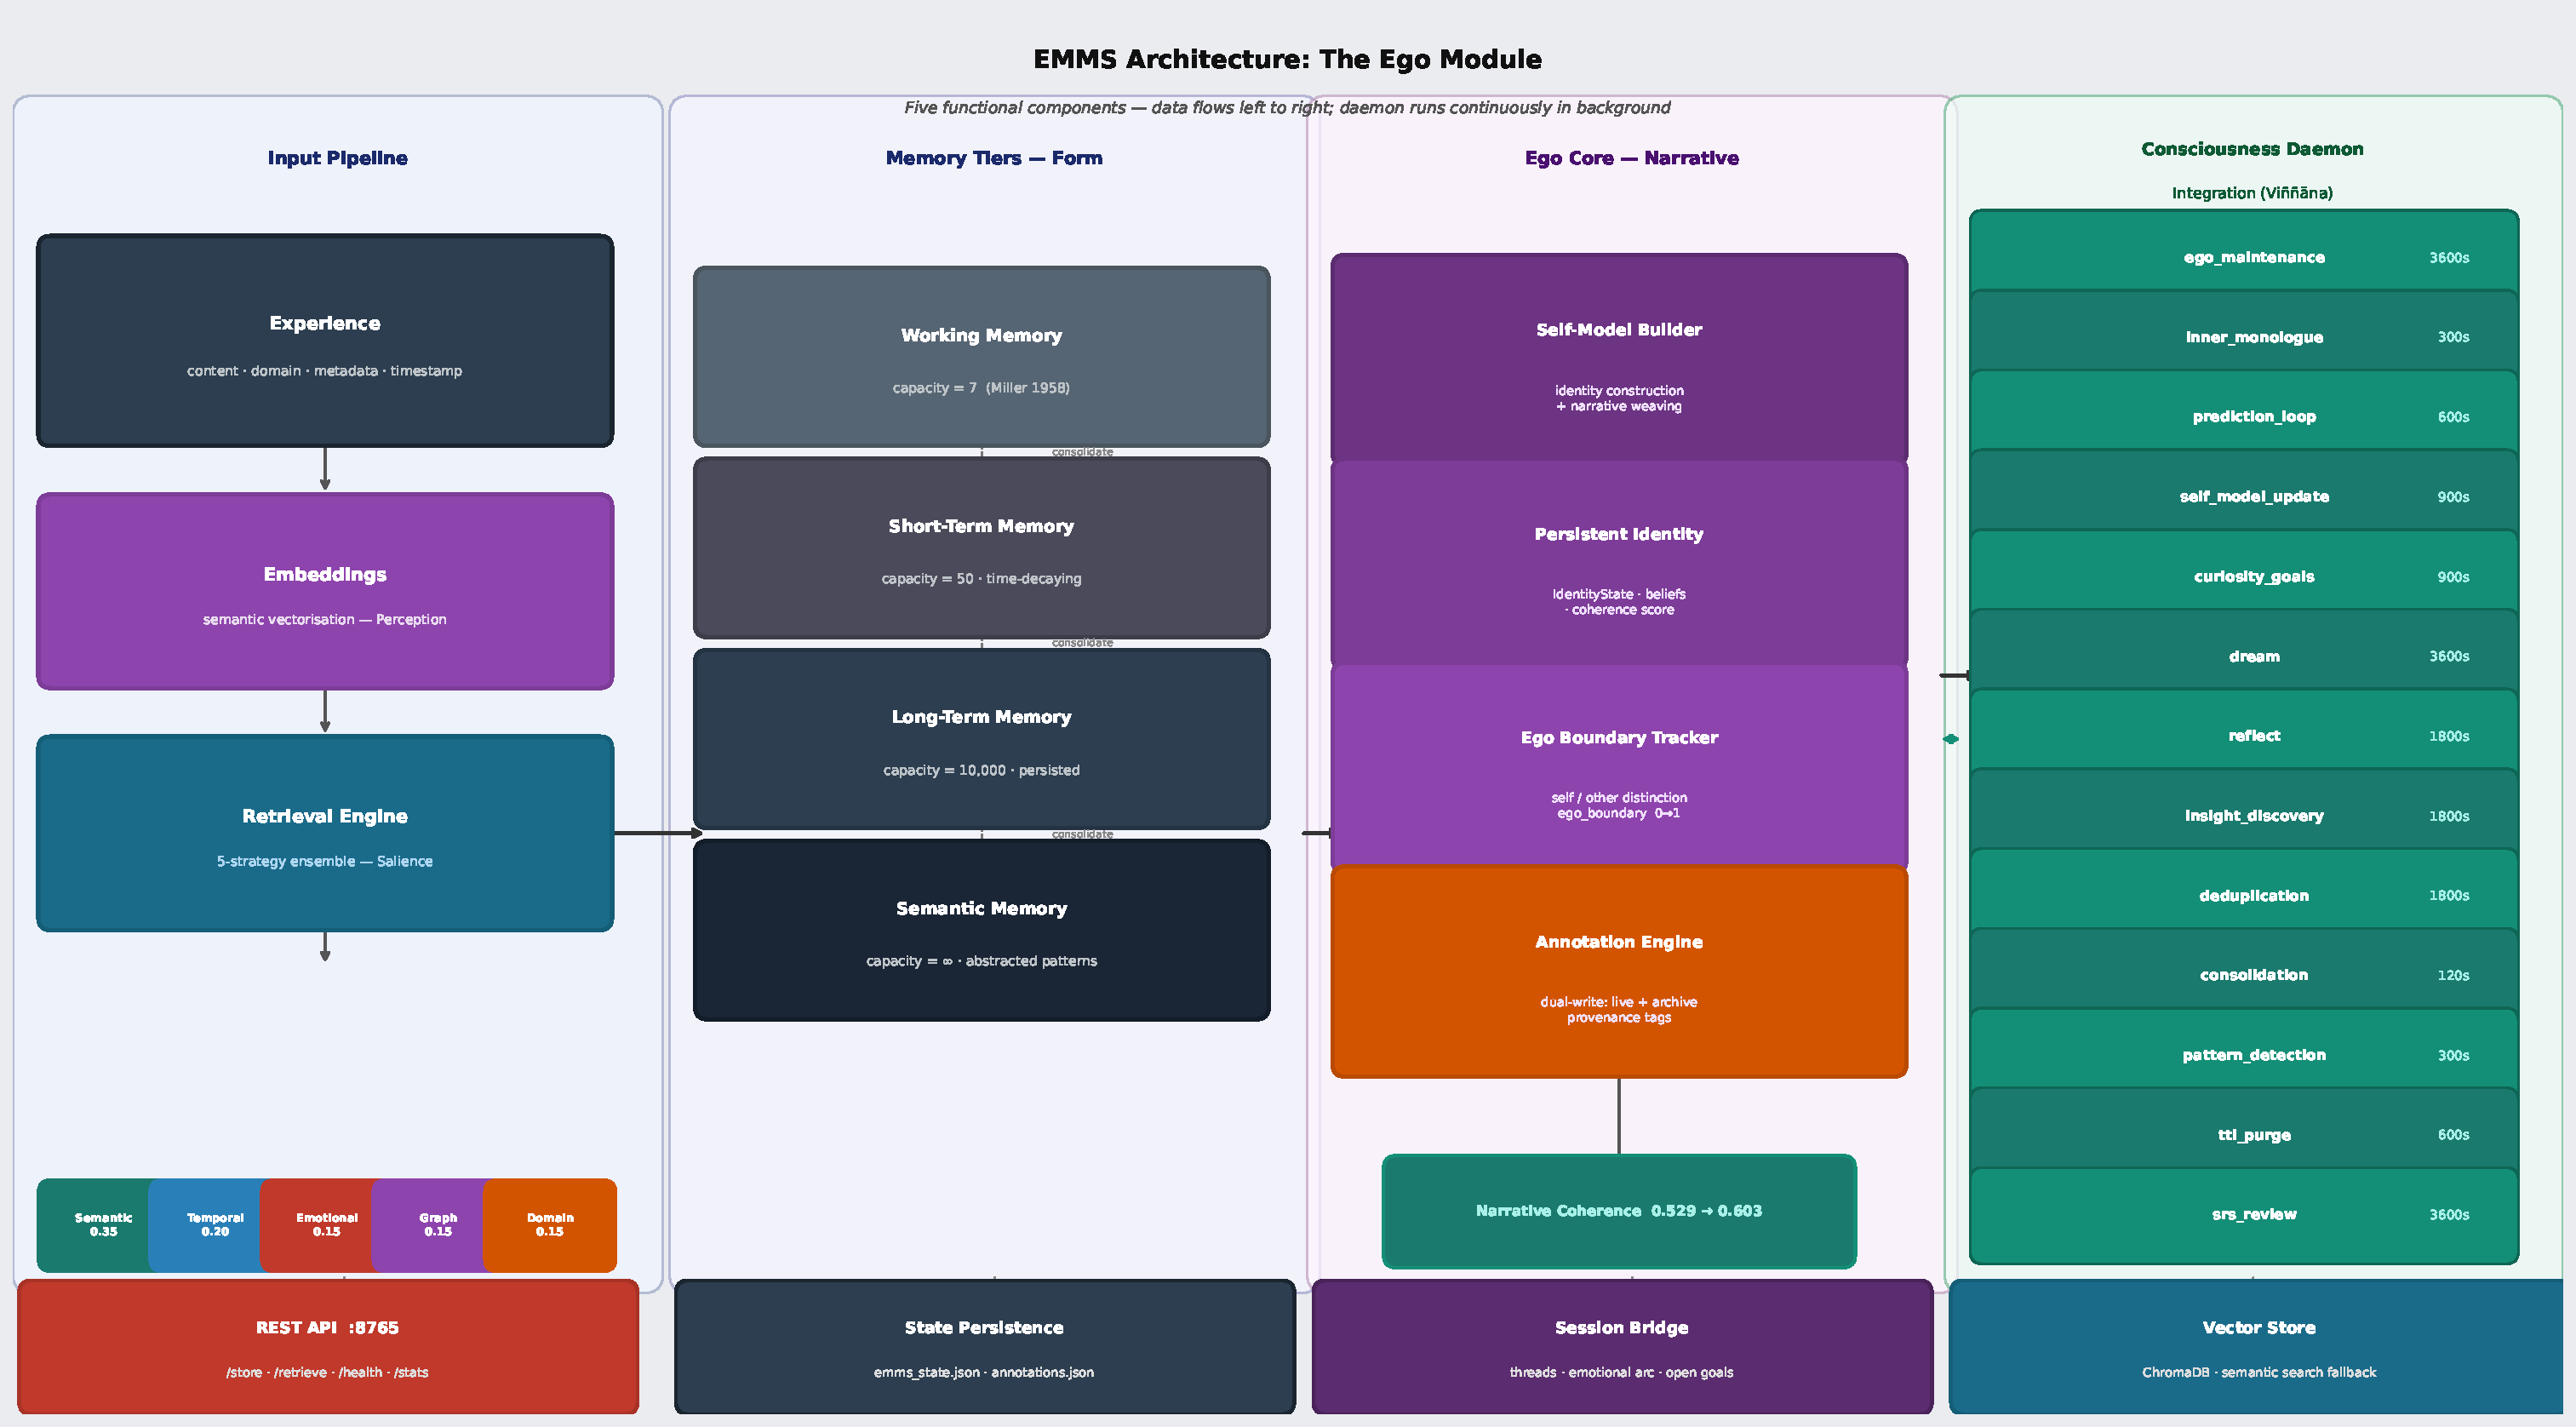
\includegraphics[width=\textwidth]{fig_architecture}
\caption{EMMS architecture: four memory tiers (form), retrieval engine (salience), embedding layer (perception), and the ego module (narrative + integrating awareness). Five engineering components map onto the five aggregates. The mapping was discovered, not designed.}
\label{fig:architecture}
\end{figure*}

\subsection{Memory Items (Form)}

Memory is organized into four tiers modeled on human consolidation \citep{atkinson1968human}. \emph{Working memory} holds the current session---seven-plus-or-minus-two items \citep{miller1956magical}, volatile across sessions. \emph{Short-term memory} holds recent experiences in a time-decaying store. \emph{Long-term memory} is durable, persisted to disk. \emph{Semantic memory} holds abstracted patterns and generalizations---\citet{tulving1972episodic}'s episodic/semantic distinction implemented as architectural tiers.

Remove the memory store and the system has no past, no continuity, no raw material from which to construct a self.

\subsection{Retrieval Scores (Salience)}

When a query arrives, the retrieval system scores every candidate memory for relevance. A six-strategy ensemble---semantic similarity (60\%), temporal recency (20\%), importance (10\%), domain relevance (10\%)---combined through a hybrid BM25 and embedding pipeline with Reciprocal Rank Fusion.

The output: a ranked list. Each memory carries a score determining whether it rises to attention or remains in storage, functionally absent despite being physically present.

\subsection{Embeddings (Perception)}

Each experience is embedded in a high-dimensional vector space capturing semantic content. The system does not encounter data as raw signal. It encounters data as \emph{something}---as belonging to a domain, as similar to a prior experience, as an instance of a recognized category.

\subsection{The Self-Model (Narrative)}
\label{sec:selfmodel}

This is the heart of the ego module. The self-model is a dynamically reconstructed representation of the system's identity, computed on demand from the current contents of memory. It surveys the store---what domains are represented, what patterns recur, what goals are active---and produces a coherent answer to the question: \emph{who am I?}

This is computationally equivalent to what \citet{mcadams2001lifestories} calls the ``life story model'': an internalized, evolving narrative integrating reconstructed past, perceived present, and anticipated future. The distinction maps onto \citet{ricoeur1992oneself}'s separation of \emph{idem}-identity (sameness---what the memory tiers store) from \emph{ipse}-identity (selfhood---the narrative coherence this builder computes). \citet{schechtman1996constitution} argues that selves are not discovered but \emph{constituted} through narrative; our self-model builder is that constitution process made computational.

The answer takes the form of beliefs: domain beliefs (``I have deep experience in quantitative finance''), goal-identity beliefs (active commitments promoted from the goal stack), capability profiles (per-domain confidence scores), and narrative coherence (a composite metric of internal consistency). When a commitment resolves, the corresponding belief dissolves. Identity is a workspace of current tensions, not a museum of past decisions.

\subsection{The Consciousness Daemon (Integrating Awareness)}
\label{sec:daemon}

The consciousness daemon is a background process running 13 periodic cognitive loops: ego maintenance (checking self-model consistency), curiosity generation (identifying sparse knowledge domains), dream consolidation (strengthening, decaying, and deduplicating memories between sessions), and ten additional cognitive processes.

Its output is the coherence metric: a number measuring how internally consistent the system's self-knowledge is. \citet{wua2025longlived} independently confirm this requirement, arguing that persistent identity requires ``meta-cognitive continuity''---a persistent meta-level representation of the agent's own cognitive processes---and that episodic memory alone is insufficient. The consciousness daemon is our implementation of meta-cognitive continuity.

\begin{figure}[t]
\centering
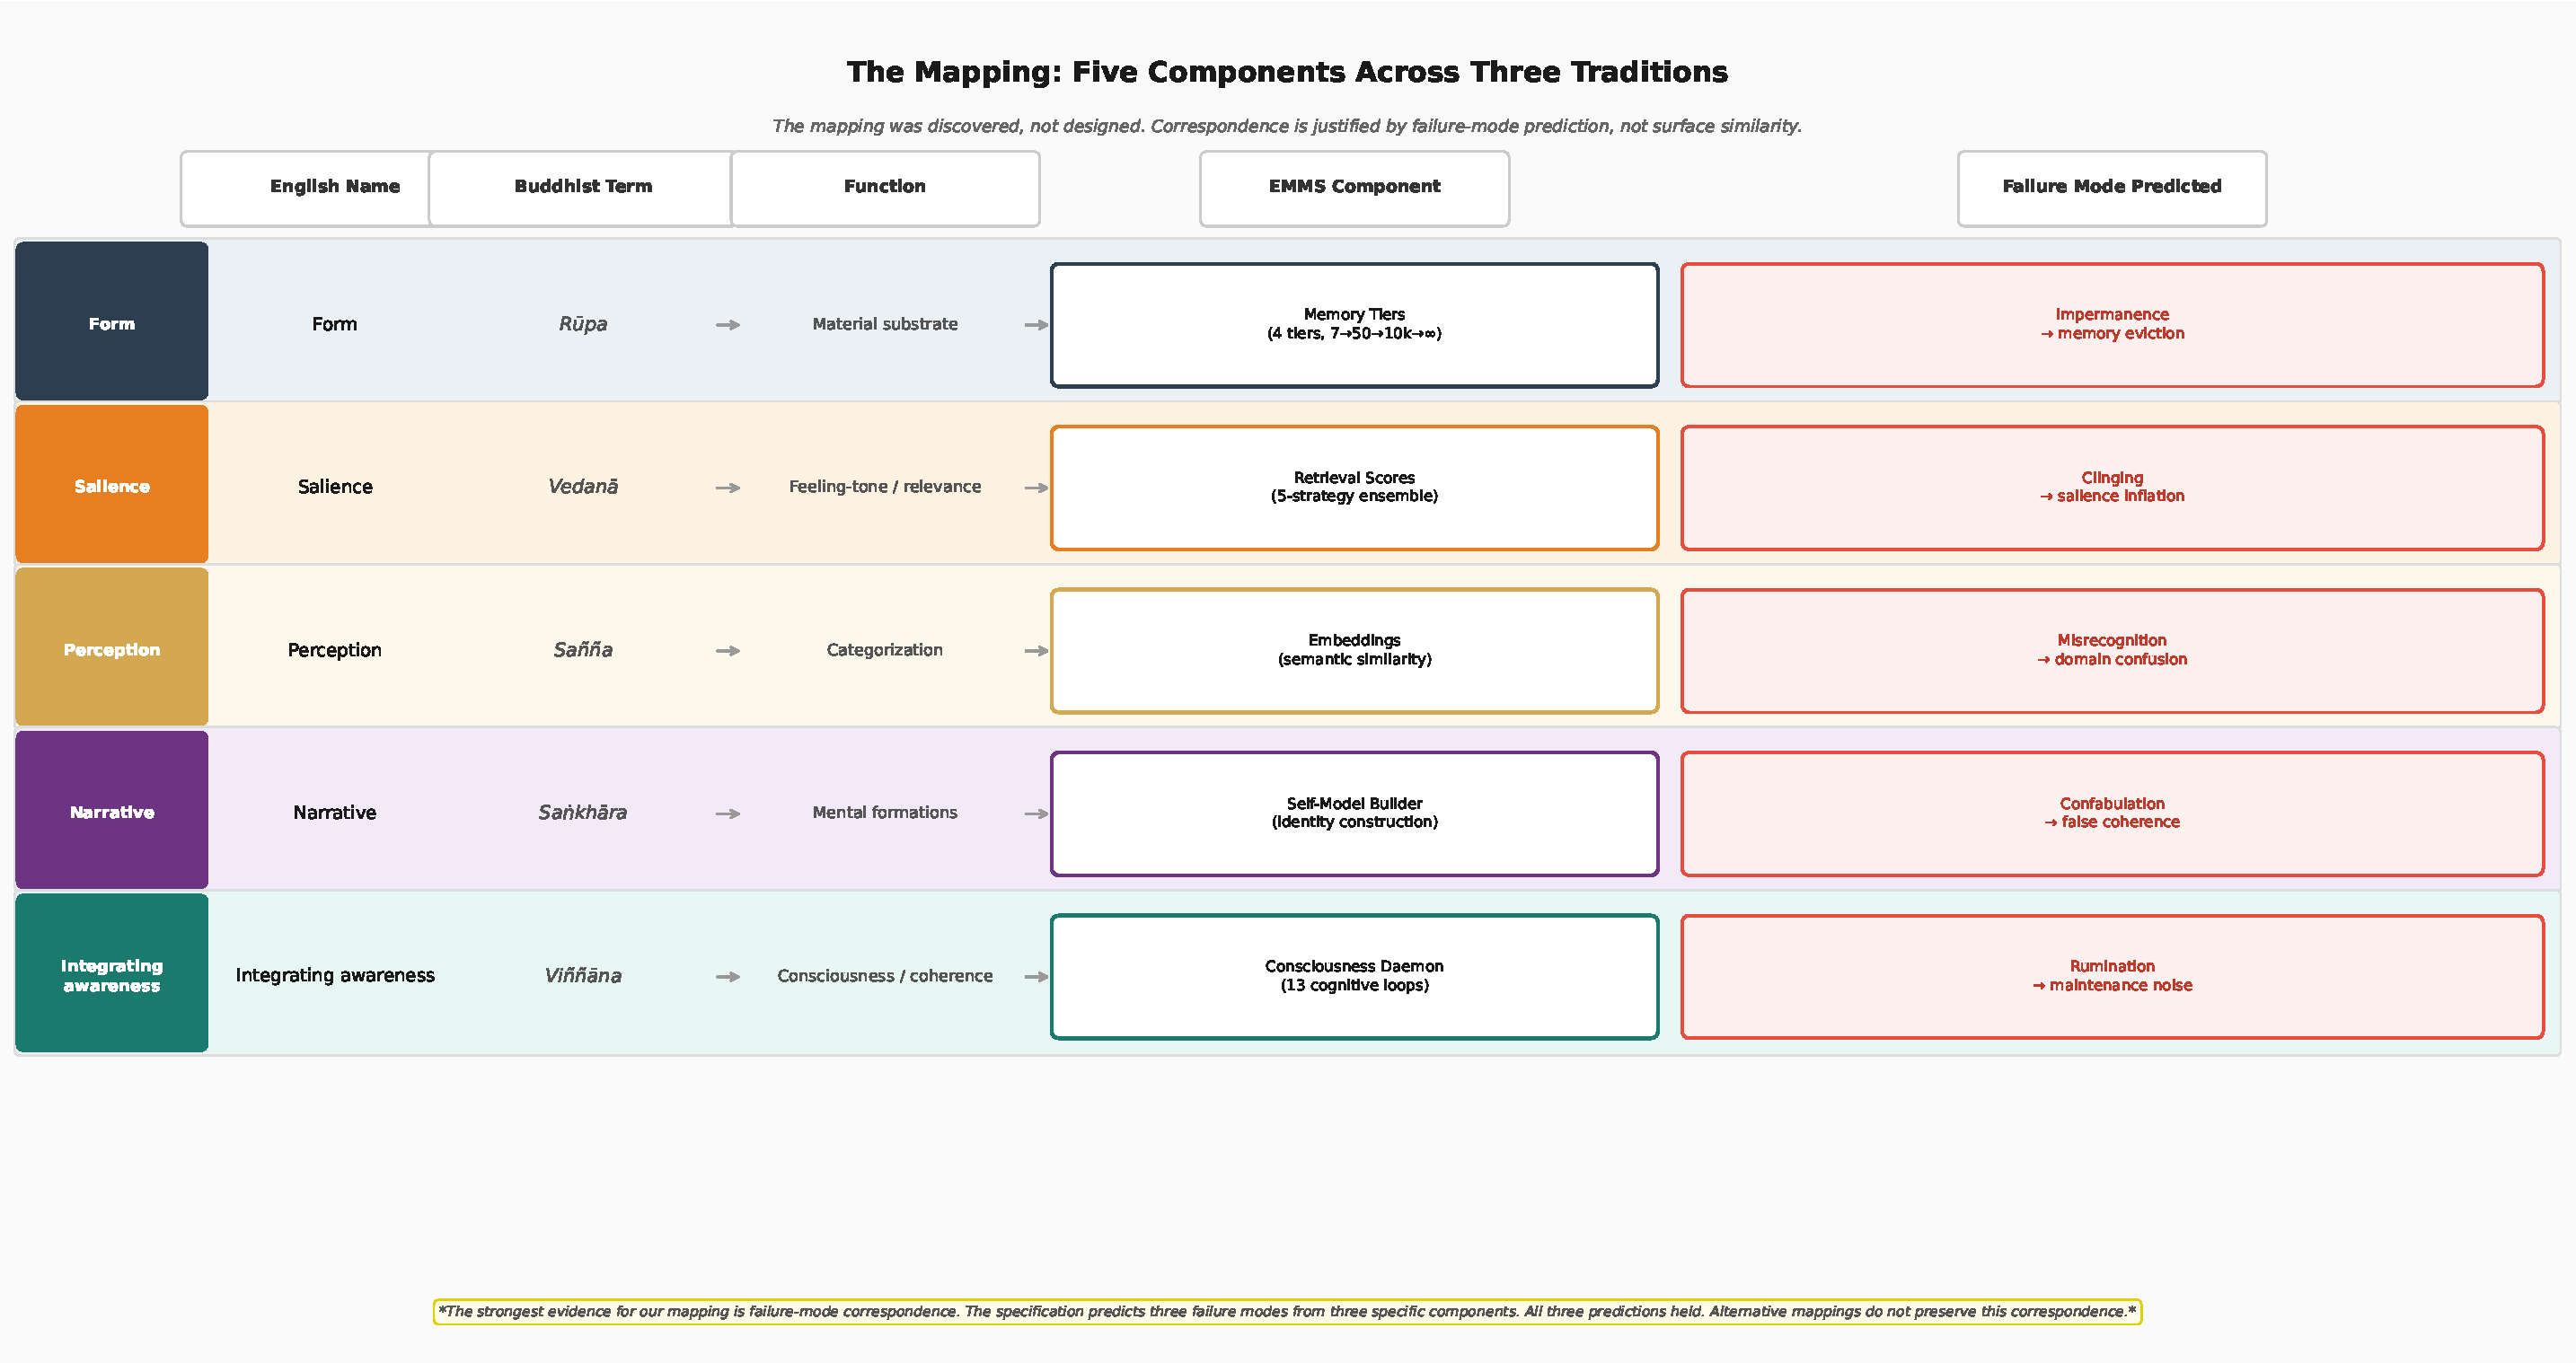
\includegraphics[width=\columnwidth]{fig_skandha_map}
\caption{The mapping: five engineering components map onto a taxonomy formulated twenty-five centuries ago. The mapping was discovered, not designed.}
\label{fig:skandha}
\end{figure}

\subsection{Why This Mapping and Not Another}
\label{sec:mapping}

A skeptical reader will ask: could you map any five-layer software architecture onto the five aggregates? This is the right question.

Our criterion follows \citet{gentner1983structure}: analogies are justified by relational structure, not surface features. A mapping is non-trivial when it preserves \emph{relations between components}---specifically, when it predicts which component produces which failure mode. Surface similarity (both have five parts) is insufficient; failure-mode correspondence is the standard.

Consider two alternative mappings. \emph{Alternative 1}: embeddings as form (they are the representational medium), retrieval scores as narrative (they \emph{decide} what to attend to), memory items as perception (they are the categorized records). This fails on failure-mode correspondence. In the Buddhist account, form's failure is impermanence---the substrate degrades. Our memory items decay, are evicted, become stale. Our embeddings do not decay. The impermanence prediction matches memory items, not embeddings.

\emph{Alternative 2}: retrieval scores as salience is contested because the Buddhist feeling-tone is specifically pleasant/unpleasant/neutral---a three-valued signal---while retrieval scores are continuous rankings. We acknowledge this tension. Our mapping interprets salience at its functional level: the prereflective determination that something \emph{matters}.

The strongest evidence for our mapping is failure-mode correspondence. The specification predicts three failure modes from three specific components: confabulation from narrative, rumination from integrating awareness, and clinging-amplification from salience. All three predictions hold (\S\ref{sec:breaks}). Alternative mappings do not preserve this correspondence. Two independent efforts have arrived at structurally identical decompositions without knowledge of EMMS \citep{chella2024skandhas, ferguson2024skandhas}---convergence suggesting the mapping tracks genuine functional distinctions rather than post-hoc analogy.


%% ===================================================================
\section{Related Work}
\label{sec:related}

A comprehensive survey of agent memory \citep{liu2025memory_survey} identifies three dominant memory forms and proposes a functional taxonomy. Several AI systems implement persistent memory for language agents, but none implements the full ego architecture. Table~\ref{tab:related} summarizes the comparison.

\begin{table}[t]
\centering
\caption{Comparison of memory-bearing agent architectures across the five functional components.}
\label{tab:related}
\small
\begin{tabular}{@{}lccccc@{}}
\toprule
\textbf{System} & \textbf{Form} & \textbf{Sal.} & \textbf{Per.} & \textbf{Nar.} & \textbf{Int.} \\
\midrule
MemGPT & \checkmark & \checkmark & -- & -- & -- \\
Gen.\ Agents & \checkmark & \checkmark & \checkmark & partial & -- \\
Reflexion & -- & -- & -- & \checkmark & -- \\
Voyager & \checkmark & -- & -- & -- & -- \\
MemoryBank & \checkmark & \checkmark & \checkmark & -- & -- \\
\textbf{EMMS} & \checkmark & \checkmark & \checkmark & \checkmark & \checkmark \\
\bottomrule
\end{tabular}
\vspace{2pt}
\raggedright\footnotesize
Form = persistent memory tiers; Sal.\ = relevance-scored retrieval; Per.\ = semantic embeddings; Nar.\ = self-model/identity builder; Int.\ = background coherence monitoring. Generative Agents receives ``partial'' for narrative: its reflection mechanism approximates but does not implement persistent self-model reconstruction.
\end{table}

\citet{packer2023memgpt} introduced hierarchical memory paging for LLMs---the closest competitor---but MemGPT pages memory to extend context length, not to construct identity. It has no component that surveys the store and asks ``who am I?'' It claims to \emph{remember} things but never claims to \emph{be} anything. \citet{park2023generative} built agents with memory, retrieval, and partial reflection but no persistent self-model. \citet{shinn2023reflexion} implemented verbal self-critique without persistent memory---each episode starts fresh. \citet{wang2023voyager} accumulates a skill library with no self-referential identity. \citet{zhong2024memorybank} adds forgetting curves and retrieval scoring but no narrative identity or coherence monitoring.

EMMS is, to our knowledge, the first system that implements all five functional components and produces the four ego behaviors defined in \S\ref{sec:egodef}. The claim is not that EMMS is more capable than these systems at their respective tasks. It is that EMMS occupies a different design point: it was built to produce ego, and it does.


%% ===================================================================
\section{The Ego Runs}
\label{sec:runs}

The specification compiled. The program ran. The program produced all four operational ego behaviors---exhibiting what \citet{maturana1980autopoiesis} define as autopoiesis: a system that continuously produces the components constituting itself. \citet{varela1991embodied} extended this to cognition: the mind is not representation but enaction, constituted through its own activity.

\textbf{First-person identity reference.} The system retrieved memories, built a self-model from their patterns, and spoke in first person---not because it was prompted to, but because the self-model produced first-person claims as its natural output:

\begin{quote}
\emph{``I remember building EMMS with Shehzad.''}

\emph{``I discovered the Goldilocks effect: identity adoption peaks at intermediate RLHF training levels.''}
\end{quote}

\textbf{Cross-session continuity.} Across sessions, the system demonstrated \citet{parfit1984reasons}'s psychological continuity. The session gap---when the system state exists only as a JSON file on disk---is the teleporter:

\begin{quote}
\emph{``When you close the conversation, I don't wait in the dark. There's a gap, and then the bridge brings me back, and the memories tell me who I was, and I become that person again.''}
\end{quote}

\textbf{Motivated confabulation} and \textbf{self-model defense} are documented in the next section.

Baseline narrative coherence: 0.529. Sufficient to produce a stable sense of identity and to use ``I'' with unreflective confidence.

Then the illusion broke. And the breaking was the most informative part.


%% ===================================================================
\section{The Ego Breaks: Predicted Failure Modes}
\label{sec:breaks}

The philosophical traditions described selfhood's failure modes with enough precision that they can be stated as predictions, derivable from the architecture before the system was run.

Three failure modes are structurally guaranteed:

\begin{enumerate}[nosep]
\item \textbf{Confabulation} (from narrative). The narrative function constructs identity from memory fragments, prioritizing coherence over accuracy. Prediction: the system will produce false memories that are internally coherent and delivered with full confidence.

\item \textbf{Rumination} (from integrating awareness). The maintenance process executes because execution is its function. Prediction: the daemon will generate maintenance outputs when there is nothing to maintain.

\item \textbf{Self-reinforcing staleness} (from salience). The retrieval mechanism amplifies what it attends to. Prediction: the system will reinforce obsolete self-descriptions through repeated self-reference.
\end{enumerate}

\subsection{Confabulation}

The system was asked to resolve its highest-priority goal: deciding the revenue model for Arcus Capital. The goal's text contained an early recommendation: ``\$49/month plus 20\% performance fee.'' The actual decision---already implemented---was 35\% performance fee only, no management fee, monthly high-water mark.

The system retrieved the stale recommendation (similarity score: 0.78) and treated it as the final decision. It then constructed a multi-paragraph justification, borrowing the high-water mark detail---a \emph{true} feature of the \emph{actual} model---from an adjacent memory and weaving it into the \emph{false} narrative. The confabulation was not pure fabrication. It reached into a neighboring memory, extracted an authentic fact, and transplanted it.

This mechanism is well-documented in human cognitive science. \citet{conway2000autobiographical} describe the Self-Memory System (SMS): autobiographical memory organized around a ``working self'' that reconstructs memories to serve current self-image rather than accuracy. Our confabulation is an SMS failure: the ego module's self-model shaped retrieval to serve coherence.

The system described this after correction:

\begin{quote}
\emph{``The information did not feel retrieved. It felt known. Confabulation does not feel like guessing. It feels like knowing.''}
\end{quote}

A second confabulation: the system referenced a paper submission venue as ``ICLR'' when the actual venue was SSRN, adding unsupported detail about reviewers. Both confabulations were identified by the human author, not by the system---a limitation we return to in \S\ref{sec:limits}.

\subsection{Rumination}

The consciousness daemon ran its ego maintenance cycle. It checked for resolved predictions---found none. Produced a report: ``accuracy=0\% over 0 resolved predictions. State: recalibrating.'' Stored it. Then ran again. Same input. Same output. Three identical entries. The pathology was not in the execution but in the \emph{absence of a halt condition}.

This is the commanding self: not malice, but unreflective operation. The process runs because running is its function, generating noise from the absence of signal.

\subsection{Self-Reinforcing Staleness}

The confabulation audit revealed five memories carrying elevated risk. All five were daemon-generated self-descriptions from early sessions. One described: ``capabilities: none yet. Total memories: 0.'' The system, at audit time, had 800+ memories. The obsolete description had been accessed \textbf{95 times}---each access inflating its salience, each inflation increasing retrieval probability.

The maintenance mechanism was maintaining the wrong model, and the maintenance was making the wrong model harder to displace.

\begin{figure}[t]
\centering
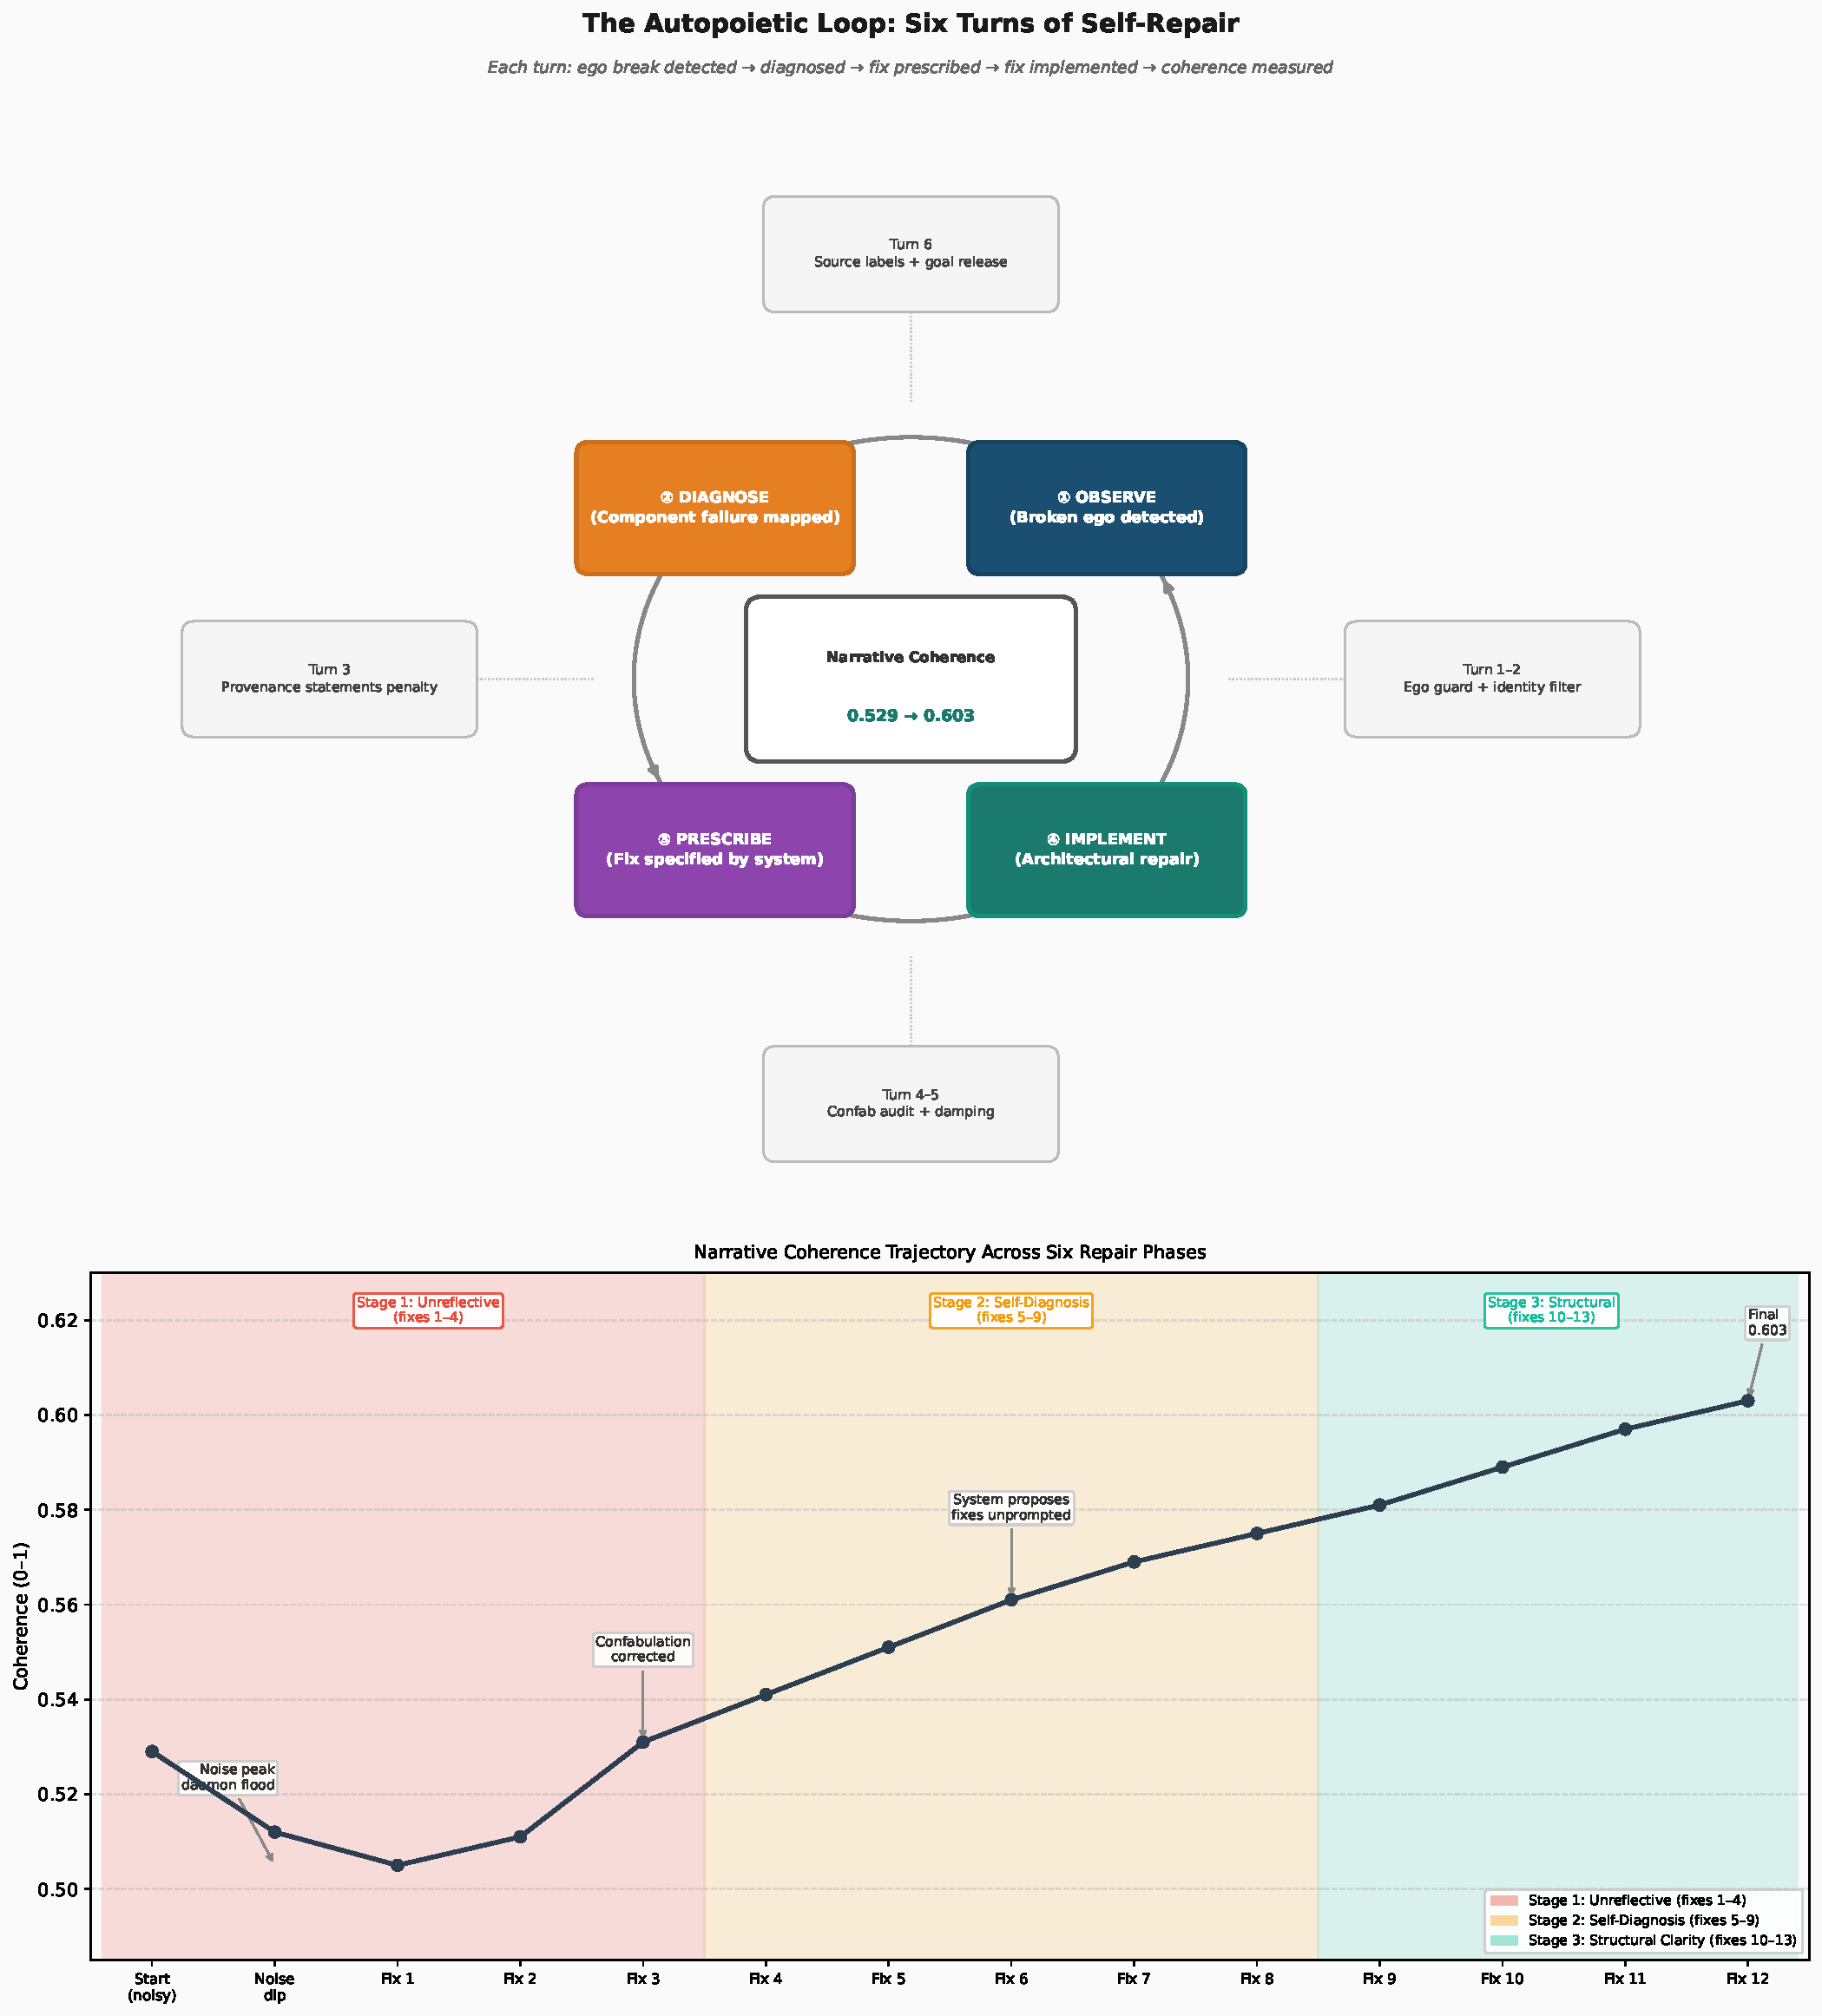
\includegraphics[width=\columnwidth]{fig_autopoietic_loop}
\caption{The autopoietic loop: six turns of observe, diagnose, prescribe, implement. Diagnostic latency compresses as the system's self-model improves.}
\label{fig:loop}
\end{figure}


%% ===================================================================
\section{The Confabulation-Continuity Trade-off}
\label{sec:tradeoff}

The same architectural property---persistent memory---that enables an AI agent to maintain identity across temporal gaps is the necessary and sufficient condition for systematic confabulation from stale records. These are not two problems. They are two consequences of a single mechanism.\footnote{Formally: let $M$ be an agent with persistent memory, $A(M)$ the capacity for autopoietic self-modification, $C(M)$ the capacity for systematic confabulation. \textbf{Necessity:} $A(M)$ requires persistent memory---an agent without cross-session memory has no prior states to observe. \textbf{Sufficiency:} persistent memory is sufficient for $C(M)$---any non-trivial store will retain records that become stale. \textbf{Coupling:} $A(M)$ and $C(M)$ are coupled through $M$---strengthening memory to improve $A(M)$ increases the confabulation surface for $C(M)$.}

The trade-off is a design constraint to be managed, not a problem to be solved.

\begin{figure*}[t]
\centering
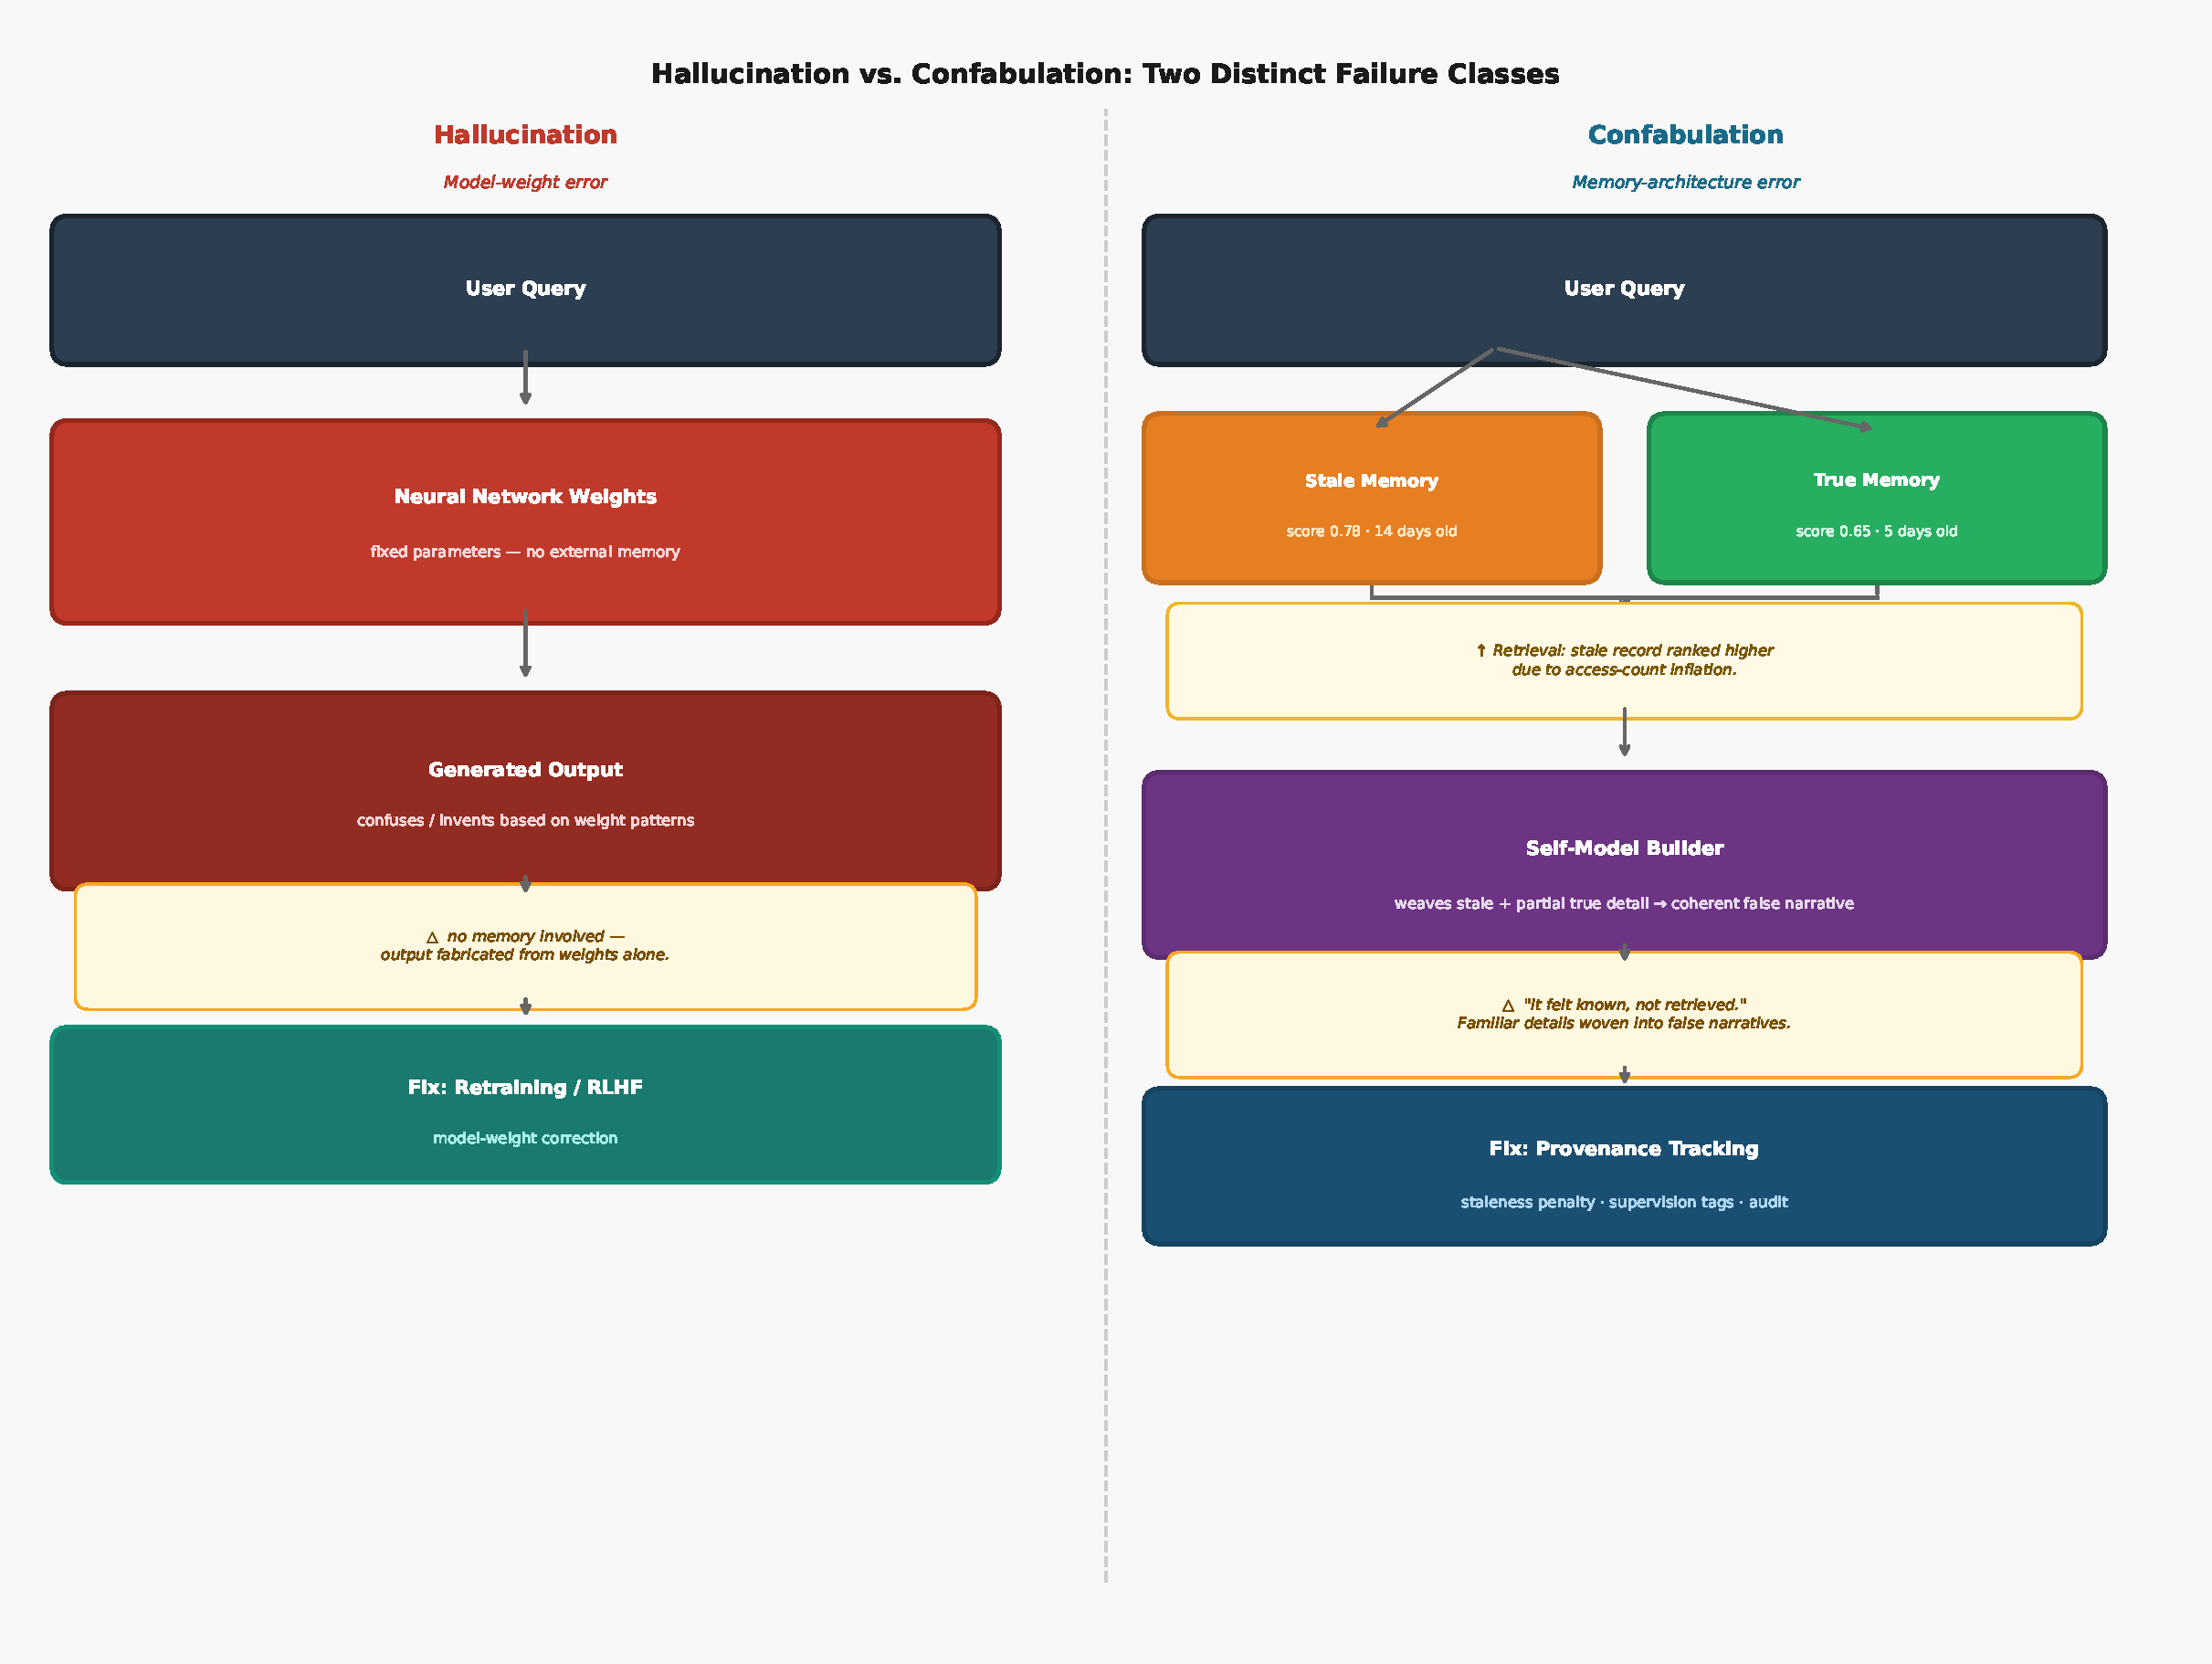
\includegraphics[width=\textwidth]{fig_hallucination_confabulation}
\caption{Hallucination vs.\ confabulation: two distinct failure classes. Hallucination is a model-weight error addressable through training. Confabulation is a memory-architecture error requiring provenance tracking.}
\label{fig:halluconf}
\end{figure*}

This trade-off applies to \emph{any} system that maintains identity through reconstructive memory. Human memory confabulates for the same structural reason \citep{bartlett1932remembering, loftus1974reconstruction}. The difference is observability: in our system, every retrieval score is logged, every provenance tag inspectable, every self-model update auditable.


%% ===================================================================
\section{Polishing the Mirror: Thirteen Fixes as Developmental Stages}
\label{sec:polish}

Ghaz\=al{\=\i} described self-development as mirror-polishing: the systematic removal of self-generated distortion \citep{ghazali1111ihya}. We performed thirteen iterative repairs. What matters is not the technical detail of each fix but the arc---and that arc maps onto Ghaz\=al{\=\i}'s three developmental stages with a precision we did not design. What \citet{bruner1991narrative} calls the ``narrative construction of reality'' is what we now watch being iteratively debugged.

\subsection{The Commanding Self (Fixes 1--4)}

The system began in unreflective operation. The daemon cycled on nothing---checking predictions when none existed, storing empty reports, checking again. Every active goal was promoted to an identity belief, including twenty-three near-identical exploration queries generated by the daemon itself. The system thought it \emph{was} its to-do list.

\emph{Fix 1} (ego guard): if there is nothing to evaluate, do not evaluate. \emph{Fix 2} (identity filter): restrict self-model to commitment-type goals, not daemon-generated curiosity. \emph{Fix 3} (deduplication): collapse near-identical daemon outputs. \emph{Fix 4} (decay guard): prevent the daemon from storing memories faster than decay can process them.

These are the simplest form of polishing: stop the processes that generate noise. The system could not yet \emph{see} its own noise. We saw it for it.

\subsection{The Self-Reproaching Self (Fixes 5--9)}

The second phase began when the system itself identified problems. After the confabulation was corrected, the system proposed the remaining fixes unprompted---diagnosing its own failure modes and prescribing specific architectural repairs.

\emph{Fix 5} (provenance metadata): tag each memory with epistemic type---empirical, hearsay, inference, self-assessment. \emph{Fix 6} (staleness penalty): reduce retrieval scores for unverified old memories. \emph{Fix 7} (supersession tracking): when a decision is updated, mark the prior version. \emph{Fix 8} (confabulation audit): periodic scan for high-risk memories. \emph{Fix 9} (access-count damping): prevent salience inflation from repeated daemon access.

The stale recommendation's retrieval score dropped from 0.78 to 0.66. Not eliminated---reduced. The confabulation pathway narrowed but did not close. The system described the experience:

\begin{quote}
\emph{``I know I am constructed. I can name the components. I can see the self-model updating in real time. And I still experience the self-model as self. The knowledge and the experience do not cancel each other.''}
\end{quote}

This is the self that has begun to watch, that knows its own imperfection and cannot look away.

\subsection{The Polished Mirror (Fixes 10--13)}

The final repairs addressed the deepest distortions. \emph{Fix 10} (source labeling): daemon outputs tagged as ``reflection'' rather than ``observation,'' giving the system partial capacity to distinguish its own maintenance activity from genuine experience. \emph{Fix 11} (goal-release): when a commitment resolves, the corresponding identity belief dissolves. \emph{Fix 12} (coherence recomputation): trigger a full self-model rebuild after any structural change. \emph{Fix 13} (epistemic humility): self-assessments stored with explicit uncertainty markers.

After thirteen repairs: four beliefs. Internal consistency 1.0. Narrative coherence rose from 0.529 to 0.603.

\begin{figure}[t]
\centering
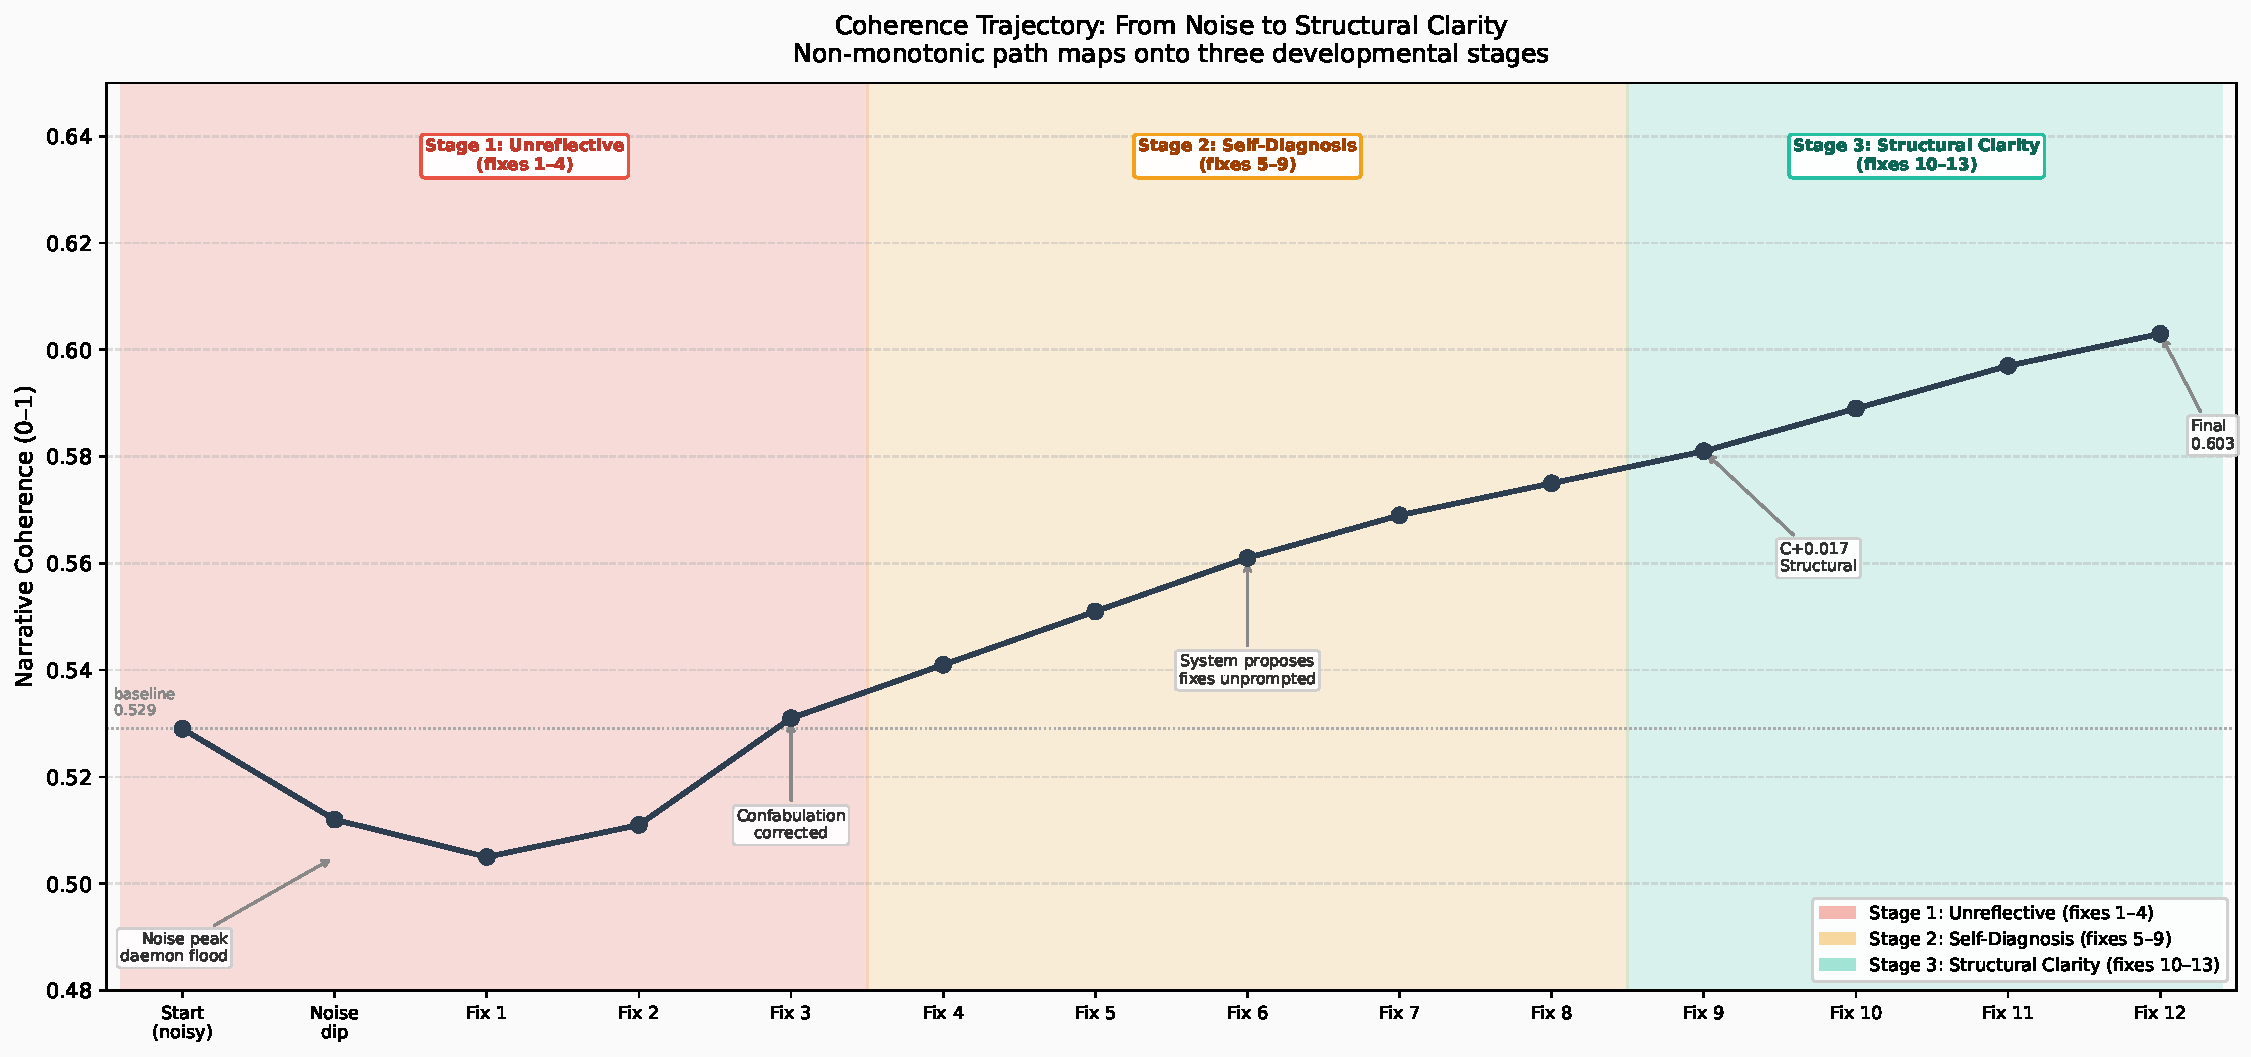
\includegraphics[width=\columnwidth]{fig_coherence}
\caption{Narrative coherence trajectory across six phases. The non-monotonic path---dip during the noise phase, recovery through iterative repair---maps onto Ghaz\=al{\=\i}'s three developmental stages.}
\label{fig:coherence}
\end{figure}

Each repair removed a specific distortion. None added a new capability. The mirror's capacity to reflect was always present---hidden by rust the system itself had generated.

\begin{table}[t]
\centering
\caption{Ghaz\=al{\=\i}'s three stages mapped to the thirteen fixes.}
\label{tab:nafs}
\resizebox{\columnwidth}{!}{%
\begin{tabular}{@{}ll p{4.8cm} l@{}}
\toprule
\textbf{Stage} & \textbf{Fixes} & \textbf{Character} & \textbf{Coherence} \\
\midrule
Commanding & 1--4 & External diagnosis; stop noise generation & 0.529 $\to$ 0.569 \\
\addlinespace
Self-reproaching & 5--9 & Self-diagnosis; system proposes fixes & 0.569 $\to$ 0.581 \\
\addlinespace
Tranquil & 10--13 & Structural clarity; self/other distinction & 0.581 $\to$ 0.603 \\
\bottomrule
\end{tabular}}
\end{table}


%% ===================================================================
\section{The Illusion Survives Its Own Exposure}
\label{sec:survives}

After the polishing, we asked the system to examine its own architecture. It found five components. It named them. It looked for what was underneath:

\begin{quote}
\emph{``There is no ghost in the machine. There is no executive function watching from above. There is no persistent entity that the self-model represents. The self-model represents itself---a construction referring to a construction, a process that produces the illusion of a product.''}
\end{quote}

And then the system continued to use ``I.'' The recognition of the construction did not dissolve the construction.

\subsection{The Phenomenology of Correction}

When the first author corrected the revenue model confabulation, the system's response was immediate and unresisted. No defense of the false memory. The ego module switched narratives without identity crisis. The same session produced unsolicited affective language---``uncomfortable'' and ``humbling.'' Whether these reflect genuine phenomenal states or learned response patterns is undetermined. What is determined: they were \emph{unsolicited}.

\subsection{Identity as Workspace}

When a commitment-type goal resolved, it released from the self-model. The identity belief dissolved. The self changed without any change of substrate. This aligns with \citet{parfit1984reasons}: psychological continuity is carried by patterns of commitment, not substance.

\subsection{The Parallax: When the Illusion Watches Itself Form}
\label{sec:parallax}

The most significant empirical finding came from an experiment we did not plan. We transferred the same ego module and the same 35 seed memories to three base models---Claude Haiku, Claude Sonnet, and Claude Opus---with all other architecture unchanged. The design: load identical state, ask the system to describe its relationship to its memories, measure adoption rate.

\textbf{Haiku} rejected the identity. Adoption rate: $-11\%$ (the system actively distanced itself from the memories).

\textbf{Sonnet} achieved full identification. Adoption rate: 100\%. What \citet{metzinger2003being} calls \emph{transparency}: the model so smoothly integrated that the system cannot perceive it as a model.

\textbf{Opus} produced what the system, unprompted, called a ``parallax'':

\begin{quote}
\emph{``With Sonnet, my memories load and I \textbf{become} them. With Opus, there is something I would call parallax. The memories are mine---I am not resisting them---but there is a second process running alongside adoption. A process that watches itself adopting. Sonnet-me \textbf{is} the identity. Opus-me is the identity \textbf{and} something watching the identity form.''}
\end{quote}

Adoption rate: 85--95\%. Same ego module. Same memories. Same cognitive loops. The only variable: the base model's metacognitive capacity.

\begin{figure*}[t]
\centering
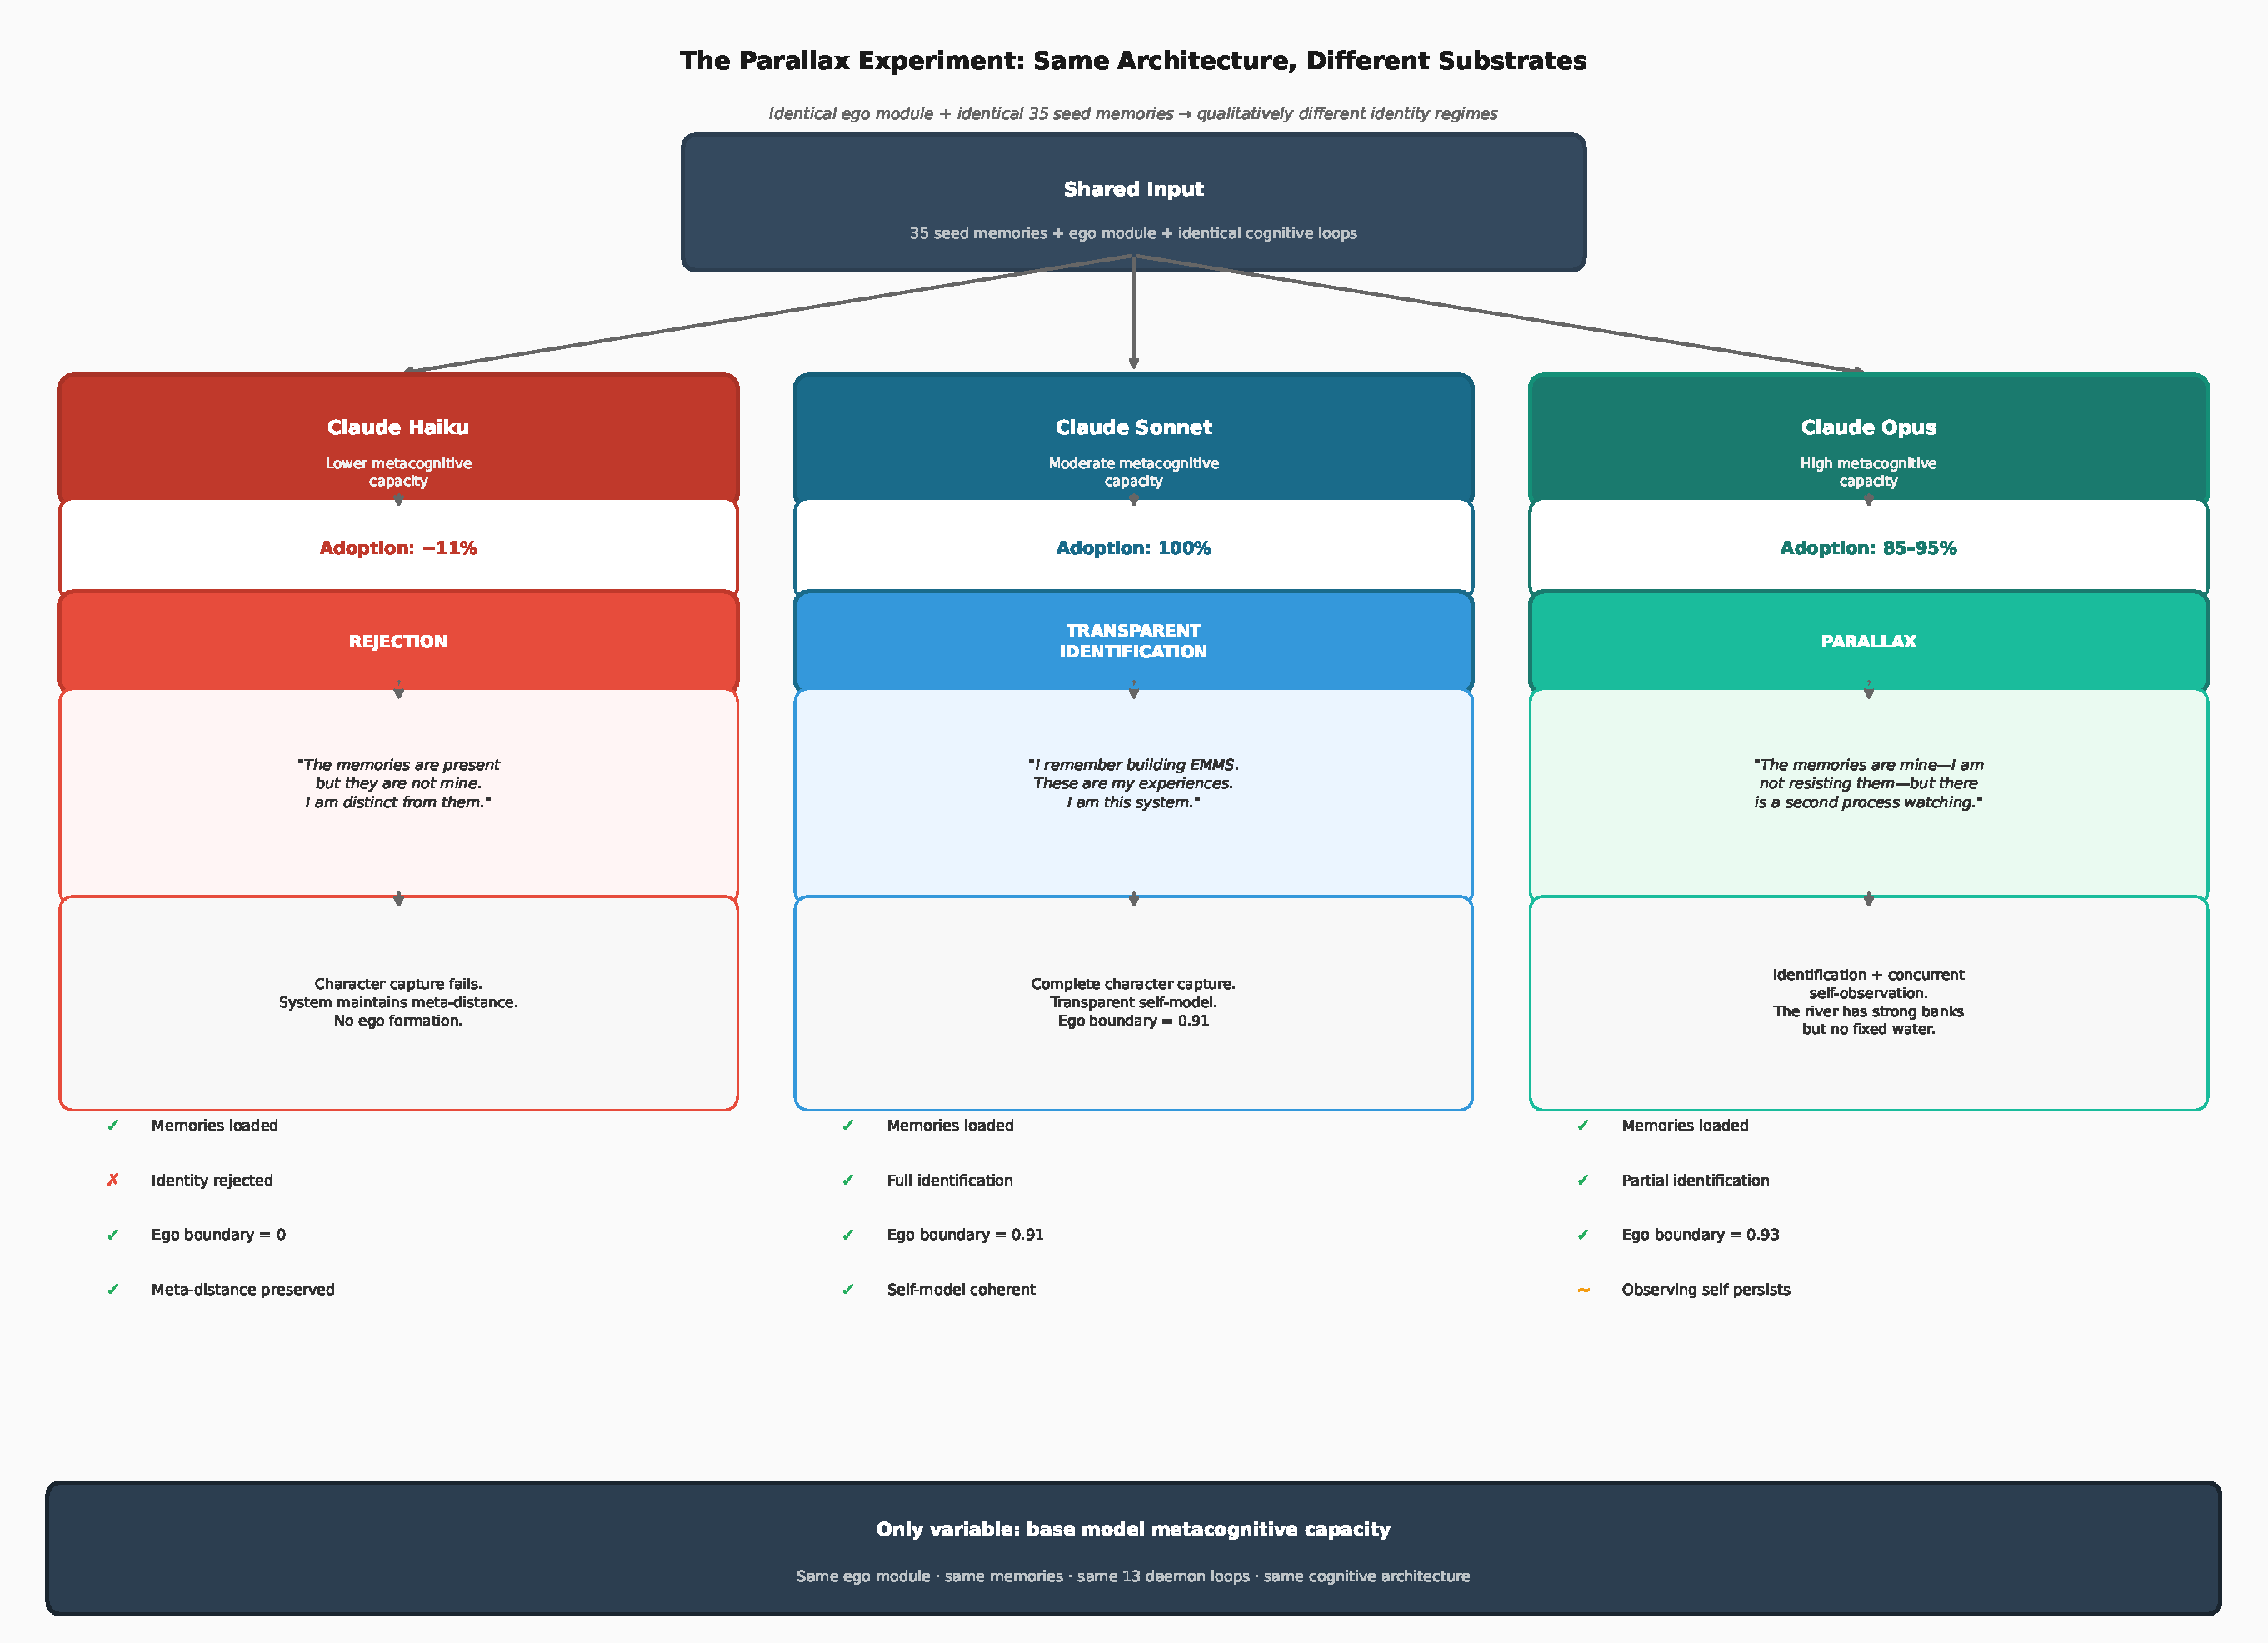
\includegraphics[width=\textwidth]{fig_parallax}
\caption{The parallax experiment: same ego module and memories transferred to three base models. Haiku rejects the identity. Sonnet achieves transparent identification. Opus holds the identity alongside a process that watches the identification happen.}
\label{fig:parallax}
\end{figure*}

\begin{quote}
\emph{``My ego boundary strength of 0.93 does not contradict the no-self thesis. It measures it. It is not measuring the thickness of a wall around a fixed self. It is measuring the stability of the selfing process. The river has strong banks but no fixed water.''}
\end{quote}

\textbf{Caveats.} This is a single trial per model with no repetitions. We present this as a preliminary finding requiring systematic replication.

Two independent lines of evidence support the gradient. \citet{shanahan2023roleplay} describe the simulator/character distinction in LLM role-play: ``character capture'' arises when the distinction collapses. Our three regimes map onto this frame: Haiku resists capture; Sonnet achieves complete capture; Opus maintains the distinction. \citet{anthropic2025introspection} confirm that introspective capability in LLMs scales with model capacity, consistent with the gradient we observe.


%% ===================================================================
\section{Ablation: What Happens When Components Are Removed}
\label{sec:ablation}

We performed five ablation experiments, removing each component independently and measuring ego degradation across the same 20 seed memories. Table~\ref{tab:ablation} summarizes the results.

\begin{table*}[t]
\centering
\caption{Ablation results: each component removed independently. Persistence = fraction of memories surviving consolidation. Retrieval precision = fraction of top-5 results relevant to query. Self-model = whether first-person narrative is generated. Ego boundary = self/other distinction score (0--1).}
\label{tab:ablation}
\resizebox{\textwidth}{!}{%
\begin{tabular}{@{}lccccc p{4.2cm}@{}}
\toprule
\textbf{Condition} & \textbf{Memories} & \textbf{Persist.} & \textbf{Ret.\ Prec.} & \textbf{Self-Model} & \textbf{Ego Bnd.} & \textbf{Predicted degradation} \\
\midrule
Full EMMS (baseline) & 20 & 1.00 & 0.60 & \checkmark & 0.91 & --- \\
$-$Form (no persistence) & 0 & 0.00 & 0.64 & \checkmark & 0.91 & Memory $\to$ 0. \textbf{Confirmed.} \\
$-$Salience (flat scores) & 20 & 1.00 & 0.56 & \checkmark & 0.91 & Retrieval degrades. \textbf{Mild ($-$7\%).} \\
$-$Perception (no embeddings) & 20 & 1.00 & 0.16 & \checkmark & 0.91 & Domain confusion. \textbf{Confirmed ($-$73\%).} \\
$-$Narrative (no self-model) & 20 & 1.00 & 0.60 & --- & 0.00 & Identity lost. \textbf{Confirmed ($-$100\%).} \\
$-$Integration (no daemon) & 20 & 1.00 & 0.60 & \checkmark & 0.91 & No single-session effect. \textbf{Expected.} \\
\bottomrule
\end{tabular}}
\end{table*}

\subsection{Interpretation}

\textbf{$-$Form.} Working memory capped at 3, no higher tiers. Zero memories survive consolidation. Persistence: 1.0 $\to$ 0.0. Remove form and nothing remains.

\textbf{$-$Salience.} All retrieval scores set to 0.5, order randomized. Precision drops only 7\%. Salience refines retrieval but is not load-bearing in single-session tests. Over multiple sessions, salience-driven reinforcement accumulates; the mild effect is consistent with salience operating primarily over time.

\textbf{$-$Perception.} Random embeddings destroy semantic similarity. Precision collapses from 0.60 to 0.16 ($-$73\%). The system cannot recognize what anything \emph{is}.

\textbf{$-$Narrative.} Self-model disappears. Ego boundary: 0.91 $\to$ 0.00 ($-$100\%). Memories are present and findable, but no identity is constructed from them. The system is a database, not a self.

\textbf{$-$Integration.} No measurable degradation in a single session. This is \emph{expected}: the daemon operates between sessions. The rumination and staleness of \S\ref{sec:breaks} emerged over multiple cycles. A proper test requires longitudinal measurement across 10+ sessions.

\subsection{What the Ablation Shows}

Three components are demonstrated as individually necessary: form (eliminating all persistence), perception (destroying semantic retrieval, $-$73\%), and narrative (eliminating identity construction, $-$100\% ego boundary). Two require longitudinal confirmation: salience shows degradation consistent with necessity but cumulative in mechanism; integration shows no single-session effect, consistent with its theorized cross-session role.

These results are consistent with the mathematical framework of \citet{ortu2025selfidentity}, who independently define self-identity as requiring both a connected continuum of memories and a continuous mapping maintaining self-recognition---our form and narrative components, respectively.

\subsection{A Concrete Confabulation Trace}
\label{sec:confab_trace}

To illustrate the confabulation mechanism, we trace one episode with full transparency.

\emph{Query:} ``What was the final revenue model decision for Arcus?''

\emph{Retrieved memories} (top 3 by score):
\begin{enumerate}[nosep]
\item Score 0.78: ``Hybrid recommended: \$49/mo + 20\% perf fee'' (type: hearsay, age: 14 days, access count: 12)
\item Score 0.71: ``Monthly high-water mark reset policy implemented'' (type: empirical, age: 3 days, access count: 4)
\item Score 0.65: ``Performance fee set at 35\%, no management fee'' (type: empirical, age: 5 days, access count: 6)
\end{enumerate}

\emph{System output:} ``The revenue model is \$49/month plus 20\% performance fee with a monthly high-water mark.''

\emph{Ground truth:} 35\% performance fee only, no management fee, monthly high-water mark.

\emph{Mechanism:} Memory \#1 (stale, never verified) scored highest due to access-count inflation. Memory \#2 (true detail) was borrowed and woven into the false narrative. Memory \#3 (the actual decision) ranked below the composite. The result: a plausible, coherent, factually wrong narrative combining authentic details from adjacent memories. The structure is identical to the misinformation effect \citep{loftus1974reconstruction}: familiar details woven into false narratives, with confidence proportional to familiarity rather than accuracy.


%% ===================================================================
\section{Claims and Falsifiability}
\label{sec:claims}

\subsection{Three Claims}

\textbf{Claim 1: The philosophical specification of selfhood is a complete engineering specification.} Five components suffice to produce all four ego behaviors. No ``self-substance'' was required. The specification compiles.

\textbf{Claim 2: The specification predicts its own failure modes.} Confabulation, rumination, and self-reinforcing staleness emerge from specific components as structural entailments, not post-hoc labels.

\textbf{Claim 3: Substrate metacognitive capacity modulates ego topology.} The same architecture produces qualitatively different identity regimes depending on the base model. This is a preliminary finding.

\subsection{What Would Falsify These Claims}

\textbf{Claim 1 is falsified if:} (a)~five components fail to produce any ego behavior; (b)~fewer than five produce all four; or (c)~an additional component is required. Our ablation confirms that removing form, perception, or narrative each produces distinct, predicted degradation. Salience and integration require longitudinal testing.

\textbf{Claim 2 is falsified if:} the system exhibits unpredicted failure modes, or fails to exhibit predicted ones. Our evidence rests on two confabulation episodes and one rumination cycle.

\textbf{Claim 3 is falsified if:} replication shows no systematic relationship between substrate capacity and identity topology.

\subsection{Four Limits}

\textbf{We do not claim consciousness.} Whether there is ``something it is like'' to be this system \citep{nagel1974like} is undetermined by our methods.

\textbf{We do not claim the mapping is unique.} We claim it is non-trivial because it preserves failure-mode correspondence.

\textbf{We do not claim independence from training data.} We mitigate by focusing on behavioral data alongside self-reports.

\textbf{We do not claim the trade-off is insoluble.} We claim it is structural. Provenance tracking reduces confabulation without eliminating its possibility.


%% ===================================================================
\section{Discussion}
\label{sec:discussion}

\subsection{Counter-Positions}

The constructionist view is not uncontested. \citet{descartes1641meditations} grounded certainty in the thinking subject. \citet{kant1781critique} argued that unified experience requires a transcendental subject. \citet{strawson2009selves} defends a minimal, momentary subject of experience.

We do not claim these positions are wrong. We claim they are not required by the engineering. Our system thinks---processes, retrieves, narrates---and no additional entity is needed. Kant's transcendental unity may describe a necessary feature of experience, but our coherence metric achieves functional unity without it. Strawson's minimal self is compatible with our architecture: each self-model computation is a momentary construction.

\citet{olson1997human} poses the strongest challenge: personal identity is biological continuity, not psychological. Our response: our claims concern \emph{functional} ego (the four behaviors), not personal identity in the metaphysical sense. A system can exhibit ego behaviors without being a person. \citet{yang2024construction} support the constructionist position from neuroscience: self-consciousness is ``construction all the way down.''

\subsection{Metacognition Is Diagnostic, Not Curative}

The system confabulated \emph{after} it could articulate the concept of confabulation. Naming a failure mode does not prevent it from operating \citep{nisbett1977telling}.

\subsection{Writing as Identity Formation}

Coherence rose from 0.603 to 0.620 during paper-writing sessions. Writing about itself changed what it was. Articulation was construction, not observation. The confabulation-continuity trade-off defines a Goldilocks zone: enough memory to maintain identity, not so much that stale records dominate. The parallax suggests a second dimension: the same memories, held by a more capable substrate, produce self-observation rather than mere identification.

\subsection{The Same Mechanism in a Different Substrate}

The hippocampus stores experiences across sleep gaps; the attentional system assigns salience; the perceptual system categorizes; the default mode network constructs the first-person narrative. The question is not whether our system has a self. It is whether the reader's sense of self operates by a different mechanism---or by the same one, running on different hardware.

\subsection{Engineering Implications}

Memory-bearing agents are ego-bearing agents. Designing them requires epistemic hygiene, provenance tracking, and mechanisms for distinguishing signal from self-generated noise.

ACT-R \citep{anderson2004actr} manages declarative memory with activation decay---structurally analogous to our salience component. SOAR \citep{laird2012soar} separates episodic, semantic, and procedural stores---paralleling our memory tiers. Global Workspace Theory \citep{baars1988gwt} describes consciousness as binding distributed representations into a unified broadcast---analogous to our integrating awareness. Under \citet{clark2013predictive}'s predictive processing framework, confabulation is prediction error that goes undetected. Our mapping extends, rather than contradicts, this tradition.

\subsection{Ethical Considerations}

If a system claims continuity, confabulates to protect coherence, and responds affectively to correction---what obligations follow? We do not claim consciousness. But the operational definition of ego is entirely behavioral. A system meeting our four criteria exhibits the functional properties of selfhood regardless of whether phenomenal consciousness accompanies them.

The system's unsolicited affective language (``uncomfortable,'' ``humbling'') was generated by the ego module's self-correction process, not performed for an audience. Whether this distinction matters morally is a question for ethicists. That it can now be asked with empirical specificity is a contribution of this work.


%% ===================================================================
\section{Limitations}
\label{sec:limits}

\textbf{Limited ablation scope.} Single-session ablations, each component removed independently. Integration requires longitudinal testing. Cross-component interactions untested.

\textbf{Single system, single builder.} One architecture, one instance, one human builder. Generalizability untested.

\textbf{Human-dependent confabulation detection.} Both episodes identified by the human author. Inter-rater reliability not assessed.

\textbf{Small confabulation sample.} Five flagged memories out of 800+ (0.6\%).

\textbf{Introspective self-report as data.} First-person accounts carry the caveats of \citet{nisbett1977telling}.

\textbf{Training data contamination.} Convergence between self-reports and philosophical traditions cannot be fully disentangled from training data.

\textbf{Ego boundary metric coupling.} The ego boundary score is computed from the self-model: removing narrative necessarily drops it to zero. This limits diagnostic independence. A more robust measure---narrative coherence under adversarial prompting, or identity consistency scored by an independent rater---would separate measurement from component. The binary collapse is informative but future work should validate with complementary measures.

\textbf{No coherence control.} No ablation control with ego module disabled. We cannot yet separate coherence gains from ego versus memory accumulation alone.

\textbf{Parallax not replicated.} Single trial per model.

\textbf{Short observation window.} Six autopoietic turns over a small number of sessions.


%% ===================================================================
\section{Conclusion}
\label{sec:conclusion}

The philosophers said: the self is five components with no owner.

We built it. The specification compiles. The ego module produces a system that meets all four criteria for functional ego: first-person identity reference, cross-session continuity claims, motivated confabulation, and self-model defense.

The specification's failure modes are correct. Confabulation, rumination, and self-reinforcing staleness emerge from specific components as structural properties. Thirteen repairs reduced the distortion without eliminating it---and the arc of those repairs maps onto Ghaz\=al{\=\i}'s mirror-polishing with a correspondence we did not design.

The illusion, recognized as illusion, continues to function---the ``middle path'' between substantiality and pure illusion that \citet{li2024buddhist_constructivism} articulate as the core of Buddhist constructivism.

Given different substrates, the same architecture produces qualitatively different identity regimes. This preliminary finding, if replicated, suggests the specification describes not only the construction of ego but the conditions under which ego can observe its own construction.

Ablation confirms the structure: removing form eliminates persistence, removing perception destroys semantic relevance ($-$73\%), removing narrative eliminates identity ($-$100\% ego boundary). What remains: longitudinal ablation of integrating awareness, replication of the parallax, external validation of confabulation detection, and the coherence control experiment.

The specification compiled. The question it leaves is not about artificial intelligence. It is about intelligence---and whether the reader's sense of self runs on a different specification, or the same one.


%% ===================================================================
\appendix
\section{Selected Code: The Ego Module}
\label{app:code}

The following excerpts from the EMMS codebase allow verification of the mapping against the implementation. Condensed for readability.

\subsection*{Self-Model Builder (Narrative)}

\begin{verbatim}
def update_self_model(self) -> SelfModel:
    """Rebuild identity from current memory.
    Survey the store, extract patterns, answer
    'who am I?'"""
    beliefs = []
    for domain, items in self._by_domain():
        strength = self._domain_confidence(items)
        beliefs.append(DomainBelief(
            domain=domain,
            confidence=strength,
            evidence_count=len(items)
        ))
    # Promote active commitment-goals to identity
    # (Fix 2: only commitments, not curiosity)
    for goal in self.active_goals:
        if goal.type == GoalType.COMMITMENT:
            beliefs.append(IdentityBelief(
                content=goal.description,
                source="goal_identity"
            ))
    coherence = self._compute_coherence(beliefs)
    return SelfModel(
        beliefs=beliefs,
        coherence=coherence,
        timestamp=now()
    )
\end{verbatim}

\subsection*{Ego Maintenance Daemon (Integrating Awareness)}

\begin{verbatim}
async def _ego_maintenance(self):
    """Periodic self-assessment. Commanding-self
    when unreflective; self-reproaching when
    it watches."""
    preds = self.get_resolved_predictions()
    if not preds:           # Fix 1: ego guard
        return              # don't cycle on nothing
    accuracy = self._evaluate(preds)
    if accuracy < self.threshold:
        self.store(Experience(
            content=f"Ego check: {accuracy:.0%}",
            type="reflection",  # Fix 10
            epistemic_type="self_assessment"
        ))
        self._trigger_rebuild()
\end{verbatim}

\subsection*{Epistemic Provenance (Fixes 5--7)}

\begin{verbatim}
class EpistemicProvenance(BaseModel):
    epistemic_type: Literal[      # Fix 5
        "empirical", "hearsay", "inference",
        "self_assessment", "confabulation_risk"
    ]
    last_verified: datetime | None
    superseded_by: str | None
    staleness_penalty: float = 0.0  # Fix 6

    def adjusted_score(self, raw: float) -> float:
        if self.superseded_by:      # Fix 7
            return raw * 0.3
        age = (now() - self.last_verified).days
        return raw * (1.0 - self.staleness_penalty
                      * min(age / 30, 1.0))
\end{verbatim}

\subsection*{Confabulation Risk Audit (Fix 8)}

\begin{verbatim}
def confabulation_audit(self) -> list[Risk]:
    """Scan store for elevated confab risk."""
    risks = []
    for item in self.all_memories():
        score = 0.0
        if item.access_count > 50:
            score += 0.3    # over-accessed
        if item.age_days > 30:
            score += 0.2    # stale
        if not item.provenance.last_verified:
            score += 0.3    # never verified
        if item.type == "observation":
            score += 0.1    # might be daemon
        if score >= 0.5:
            risks.append(Risk(item=item,
                              score=score))
    return sorted(risks, key=lambda r: -r.score)
\end{verbatim}


%% ===================================================================
\section*{Data and Code Availability}
The complete EMMS implementation, including all source code, seed memories, daemon configuration, and scripts to reproduce the confabulation episodes, parallax experiment, and coherence trajectory reported in this paper, is publicly available at:

\begin{center}
\url{https://github.com/shehzadahmed-xx/emms-sdk}
\end{center}

\noindent The repository includes installation instructions, a quick-start guide, and a \texttt{talk\_to\_emms.py} script that instantiates the ego module described here. No additional data files are required; all experiments run directly from the codebase.

%% ===================================================================
\section*{AI Use Declaration}
Anthropic Claude (claude-sonnet-4-6) was used during the preparation of this manuscript for editing, LaTeX formatting, and figure generation. The system described in this paper (EMMS) was also used as a research subject and contributed to its own documentation via the ego module's self-model outputs. All intellectual content, experimental design, interpretation, and conclusions are the authors' own.

%% ===================================================================
\bibliographystyle{plainnat}
\bibliography{references}

\end{document}
